\mode*
\part{File Systems}

\lecture[fs]{fs}{fs}

\section{File System Structure}

\begin{frame}{Long-term Information Storage Requirements}
  \begin{itemize}
  \item Must store large amounts of data
  \item Information stored must survive the termination of the process using it
  \item Multiple processes must be able to access the information concurrently
  \end{itemize}
\end{frame}

\begin{frame}{File-System Structure}
  \begin{block}{File-system design addressing two problems:}
    \begin{enumerate}
    \item defining how the FS should look to the user
      \begin{itemize}
      \item defining a file and its attributes
      \item the operations allowed on a file
      \item directory structure
      \end{itemize}
    \item creating algorithms and data structures to map the logical FS onto the
      physical disk
    \end{enumerate}
  \end{block}
\end{frame}

\begin{frame}{File-System --- A Layered Design}
  \begin{minipage}{.2\textwidth}
    \begin{tblr}{colspec={c},cell{1,Z}{1}={cmd=\small\fbox}, rowsep=0pt,
      cell{3,5,7,9}{1}={cmd=\small\alert}}
      APPs\\
      $\Downarrow$\\
      Logical FS\\
      $\Downarrow$\\
      File-org module\\
      $\Downarrow$\\
      Basic FS\\
      $\Downarrow$\\
      I/O ctrl\\
      $\Downarrow$\\
      Devices
    \end{tblr}
  \end{minipage}\hfill
  \begin{minipage}{.75\textwidth}
    \begin{itemize}
    \item \alert{logical file system} --- manages metadata information
      \begin{itemize}
      \item[-] maintains all of the file-system structure (directory structure, FCB)
      \item[-] responsible for protection and security
      \end{itemize}
    \item \alert{file-organization module}
      \begin{itemize}
      \item[-] $\genfrac{}{}{0pt}{}{\text{logical block}}{\text{address}}
        \xrightarrow{translate} \genfrac{}{}{0pt}{}{\text{physical
            block}}{\text{address}}$
      \item[-] keeps track of free blocks
      \end{itemize}
    \item \alert{basic file system} issues generic commands to device driver,
      e.g
      \begin{itemize}
      \item[-] ``\texttt{read drive 1, cylinder 72, track 2, sector 10}''
      \end{itemize}
    \item \alert{I/O Control} --- device drivers, and INT handlers
      \begin{itemize}
      \item[-] \alert{device driver:}
        $\genfrac{}{}{0pt}{}{\text{high-level}}{\text{commands}} \xrightarrow{translate}
        \genfrac{}{}{0pt}{}{\text{hardware-specific}}{\text{instructions}}$
      \end{itemize}
    \end{itemize}
  \end{minipage}
\end{frame}

See also \citetitle[Sec.~1.3.5, \emph{I/O Devices}]{tanenbaum2015modern}.

\begin{frame}{The Operating Structure}
  \begin{minipage}{.25\textwidth}
    \begin{tblr}{colspec={c},cell{1,Z}{1}={cmd=\small\fbox},rowsep=0pt,
        cell{3,5,7,9}{1}={cmd=\small\alert}}
      APPs\\
      $\Downarrow$\\
      Logical FS\\
      $\Downarrow$\\
      File-org module\\
      $\Downarrow$\\
      Basic FS\\
      $\Downarrow$\\
      I/O ctrl\\
      $\Downarrow$\\
      Devices
      \end{tblr}
  \end{minipage}\quad
  \begin{minipage}{.7\textwidth}
    \begin{block}{Example --- To create a file}
      \begin{enumerate}
      \item \alert{APP} calls \texttt{creat()}
      \item \alert{Logical FS}
        \begin{enumerate}
        \item allocates a new FCB
          % \item reads the appropriate directory into memory
        \item updates the in-mem dir structure %it with the new file name and fCB
        \item writes it back to disk
        \item calls the file-org module
        \end{enumerate}
      \item \alert{file-organization module}
        \begin{enumerate}
        \item allocates blocks for storing the file's data
        \item maps the directory I/O into disk-block numbers
        \end{enumerate}
        % \item Now, to opened the newly created file
        %   \begin{enumerate}
        %   \item the given file name is searched in the directory structure
        %   \item upon found, the FCB is copied into a \alert{system-wide open-file
        %     table}
        %   \end{enumerate}
        % \item an entry is made in the \alert{per-process open-file table}
      \end{enumerate}
    \end{block}
  \end{minipage}
  \begin{block}{Benefit of layered design}
    The I/O control and sometimes the basic file system code can be used by multiple file
    systems.
  \end{block}
\end{frame}

\section{Files}

\begin{frame}{File}{A Logical View Of Information Storage}
  \begin{block}{User's view}
    \begin{itemize}
    \item[] A file is the smallest storage unit on disk.
      \begin{itemize}
      \item Data cannot be written to disk unless they are within a file
      \end{itemize}
    \end{itemize}
  \end{block}
  \begin{block}{UNIX view}
    \begin{itemize}
    \item[] Each file is a sequence of 8-bit bytes
      \begin{itemize}
      \item It's up to the application program to interpret this byte stream.
      \end{itemize}
    \end{itemize}
  \end{block}
\end{frame}

\begin{frame}{File}{What Is Stored In A File?}
  Source code, object files, executable files, shell scripts, PostScript...
  \begin{block}{Different type of files have different structure}
    \begin{itemize}
    \item UNIX looks at contents to determine type
      \begin{description}
      \item[Shell scripts] start with ``\texttt{\#!}''
      \item[PDF] start with ``\texttt{\%PDF...}''
      \item[Executables] start with \alert{magic number}
      \end{description}
    \item Windows uses file naming conventions
      \begin{description}
      \item[executables] end with ``\texttt{.exe}'' and ``\texttt{.com}''
      \item[MS-Word] end with ``\texttt{.doc}''
      \item[MS-Excel] end with ``\texttt{.xls}''
      \end{description}
    \end{itemize}
  \end{block}
\end{frame}

\begin{frame}{File Naming}
  \begin{block}{Vary from system to system}
  \begin{itemize}
  \item Name length?
  \item Characters? Digits? Special characters?
  \item Extension?
  \item Case sensitive?
  \end{itemize}    
  \end{block}
\end{frame}

\begin{frame}{File Types}
  \begin{description}
  \item[Regular files:] ASCII, binary
  \item[Directories:] Maintaining the structure of the FS
  \end{description}
  \begin{block}{In UNIX, everything is a file}
    \begin{description}
    \item[Character special files:] I/O related, such as terminals, printers ...
    \item[Block special files:] Devices that can contain file systems, i.e. disks
      \begin{description}
      \item[disks] --- logically, linear collections of blocks; disk driver translates
        them into physical block addresses
      \end{description}
    \end{description}
  \end{block}
\end{frame}

\begin{frame}
  \begin{iblock}{Binary files}
    \centering
    \mode<beamer>{ 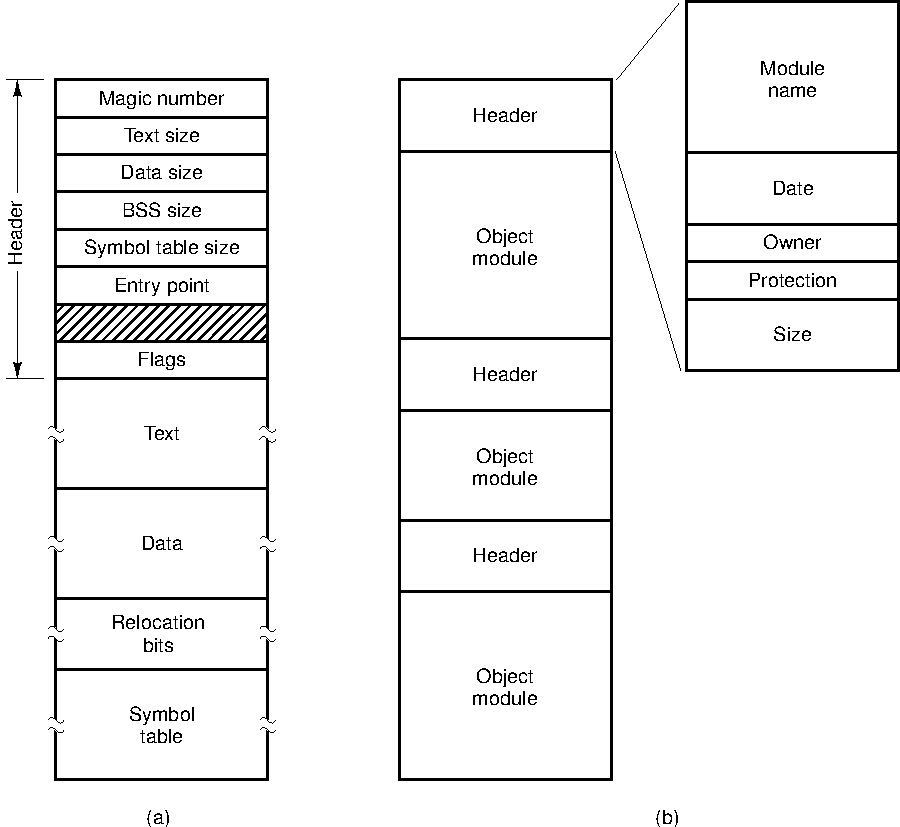
\includegraphics[width=.55\textwidth]{mos-figs-6-3} }%
    \mode<article>{ 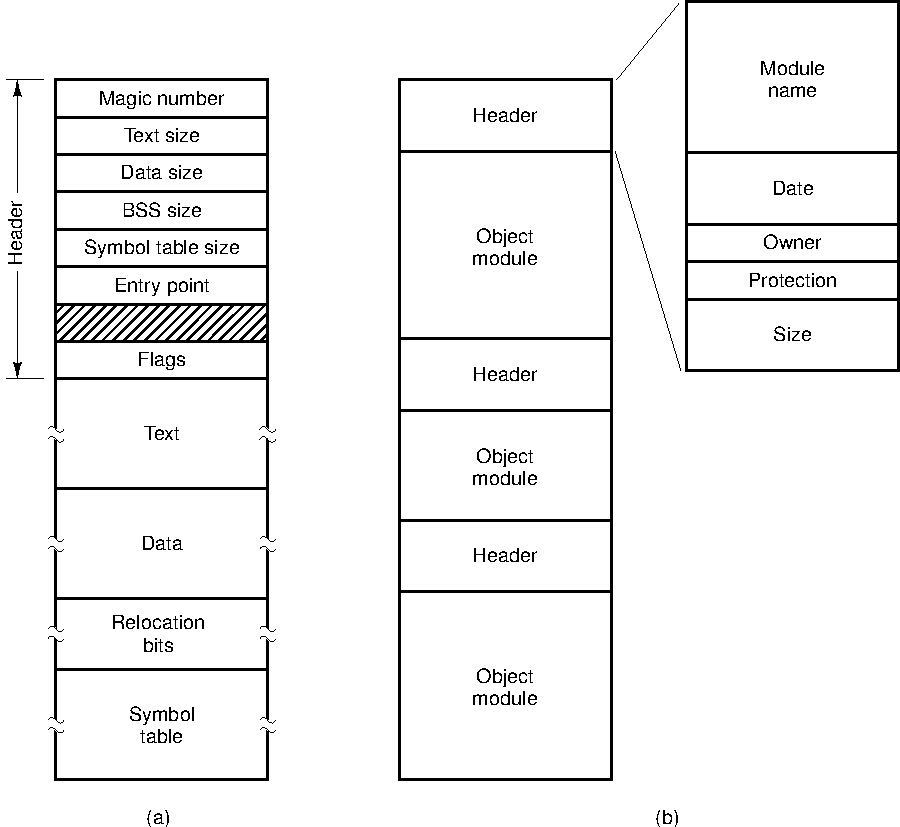
\includegraphics[width=.6\textwidth]{mos-figs-6-3} }
  \end{iblock}
\end{frame}

See also:
\begin{itemize}
\item \citetitle[\emph{Wikipedia:ELF}]{wiki:elf}.
\item OSDev: ELF\footnote{\url{http://wiki.osdev.org/ELF}}.
\end{itemize}

\begin{frame}{File Attributes --- Metadata}
  \begin{itemize}
  \item \alert{Name} - only information kept in human-readable form
  \item \alert{Identifier} - unique tag (number) identifies file within file system
  \item \alert{Type} - needed for systems that support different types
  \item \alert{Location} - pointer to file location on device
  \item \alert{Size} - current file size
  \item \alert{Protection} - controls who can do reading, writing, executing
  \item \alert{Time, date, and user identification} - data for protection, security, and
    usage monitoring
  \end{itemize}
\end{frame}

\begin{frame}{File Operations}{POSIX file system calls}%[squeeze]
  \ttfamily
  \begin{tblr}{l|l}
    creat(name, mode)&read(fd, buffer, byte\_count)\\
    open(name, flags)&write(fd, buffer, byte\_count)\\
    close(fd)&lseek(fd, offset, whence)\\
    link(oldname, newname)&chown(name, owner, group)\\
    unlink(name)&fchown(fd, owner, group)\\        
    truncate(name, size)&chmod(name, mode)\\
    ftruncate(fd, size)&fchmod(fd, mode)\\
    stat(name, buffer)&utimes(name, times)\\
    fstat(fd, buffer)&\\
  \end{tblr}
\end{frame}

\begin{frame}
  \begin{minipage}[t]{.5\linewidth}
    \begin{block}{\texttt{write()}}
      \centering
      \mode<beamer>{ \includegraphics[width=\textwidth]{write-c} }%
      \mode<article>{\cfile{../src/fs/write.c}}
    \end{block}
    \ttfamily
    \begin{itemize}
    \item[\$] man 2 write
    \item[\$] man 3 write
    \end{itemize}
  \end{minipage}\qquad
  \begin{minipage}[t]{.35\linewidth}
    \begin{block}{\texttt{read()}}
      \centering
      \mode<beamer>{ 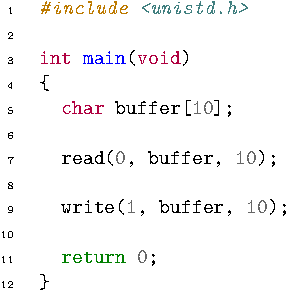
\includegraphics[width=\textwidth]{read-c} }%
      \mode<article>{\cfile{../src/fs/read.c}}
    \end{block}
    \ttfamily
    \begin{itemize}
    \item[\$] man 2 read
    \item[\$] man 3 read
    \end{itemize}
  \end{minipage}
  \vspace*{1em}
  \begin{itemize}
  \item No need to \texttt{open()} \texttt{STDIN}, \texttt{STDOUT}, and \texttt{STDERR}
  \end{itemize}
\end{frame}

\begin{frame}{\cmd{cp}}
  \centering
  \mode<beamer>{ 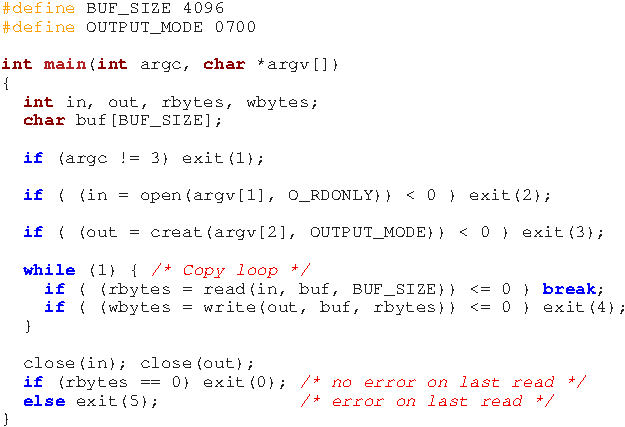
\includegraphics[height=.9\textheight]{cp-syscall-c} }%
  \mode<article>{\cfile{../src/fs/cp-syscall.c}}
\end{frame}

\begin{frame}{\texttt{stdio} --- The Standard I/O Library}
  \begin{description}
  \item[System calls:] \cmd{open(), read(), write(), close()}\ldots
  \item[Library functions:] \cmd{fopen(), fread(), fwrite, fclose()}\ldots
  \end{description}
  \begin{block}{Avoid calling syscalls directly as much as you can}
    \begin{minipage}{.4\linewidth}
      \begin{itemize}
      \item Portability
      \item Buffered I/O
      \end{itemize}
    \end{minipage}\qquad
    \begin{minipage}{.4\linewidth}
      \begin{center}
        \mode<beamer>{ 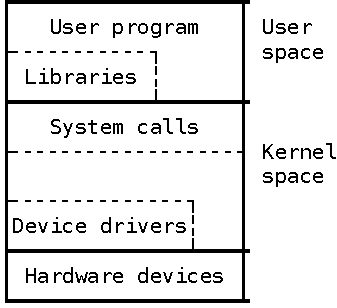
\includegraphics[width=\textwidth]{api} }%
        \mode<article>{ 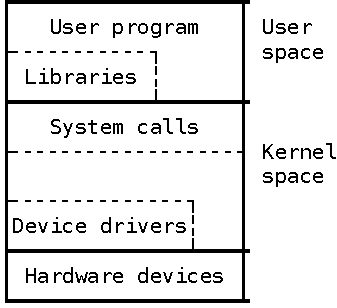
\includegraphics[width=.5\textwidth]{api} }
      \end{center}
    \end{minipage}
  \end{block}  
\end{frame}

\begin{frame}{\texttt{open()} {\scriptsize vs.} \texttt{fopen()}}
  \begin{center}
    \begin{minipage}{.48\linewidth}
      \cmd{open()}\\[1ex]
      \mode<beamer>{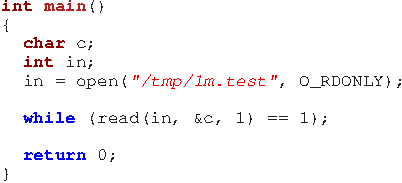
\includegraphics[width=\linewidth]{open-c}\\[1ex]}%
      \mode<article>{\cfile{../src/fs/open.c}}
      \CMD{strace -c ./open}
    \end{minipage}\quad
    \begin{minipage}{.48\linewidth}
      \cmd{fopen()} --- Buffered I/O\\[1ex]
      \mode<beamer>{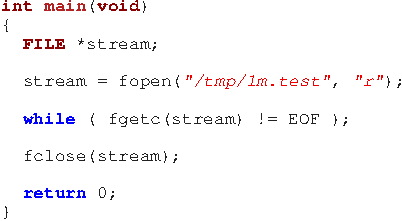
\includegraphics[width=\linewidth]{fopen-c}\\[1ex]}%
      \mode<article>{\cfile{../src/fs/fopen.c}}
      \CMD{strace -c ./fopen}
    \end{minipage}
  \end{center}{\footnotesize
  \begin{itemize}
  \item[\$] \cmd{dd if=/dev/zero of=/tmp/1m.test bs=1k count=1024}
  \end{itemize}}
\end{frame}

\begin{itemize}
\item \url{https://stackoverflow.com/questions/1658476/c-fopen-vs-open}
\end{itemize}

\begin{frame}{\texttt{cp} --- {\small With} \texttt{stdio}}
  \begin{center}
    \mode<beamer>{ 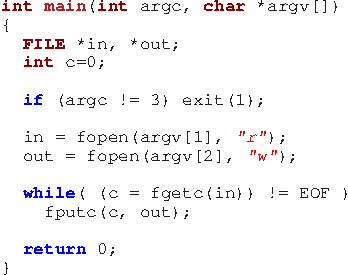
\includegraphics[width=.5\textwidth]{cp-libc-c} }%
    \mode<article>{\cfile{../src/fs/cp-libc.c}}
  \end{center}
  \begin{description}
  \item[] Try \texttt{fread()/fwrite()} instead.
  \end{description}
\end{frame}

\begin{itemize}
\item \url{https://stackoverflow.com/questions/32742430/is-getc-a-macro-or-a-function}
\item \url{https://stackoverflow.com/questions/9104568/macro-vs-function-in-c}
\end{itemize}


% \begin{frame}{Example}
%     \begin{center}
%       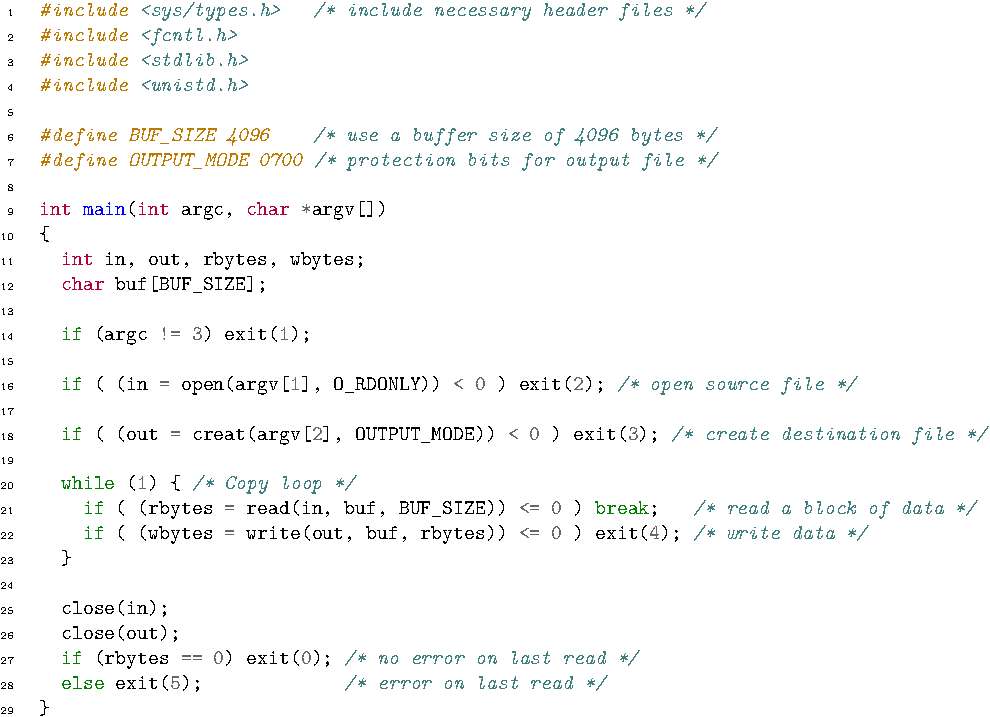
\includegraphics[width=.9\textwidth]{cp-c}
%     \end{center}
% \end{frame}

\begin{frame}{\texttt{open()}}
  \begin{block}{\texttt{fd open(pathname, flags)}}
    \begin{itemize}
    \item[] A per-process \alert{open-file table} is kept in the OS
      \begin{itemize}
      \item upon a successful \texttt{open()} syscall, a new entry is added into this table
      \item indexed by \alert{file descriptor (fd)}
      \end{itemize}
    \item[] To see files opened by a process, e.g. \texttt{init}
      \begin{itemize}
      \item[\$] \texttt{lsof -p 1}
      \end{itemize}
    \end{itemize}
  \end{block}
  \begin{block}{Why \texttt{open()} is needed?}
    To avoid constant searching
    \begin{itemize}
    \item Without \texttt{open()}, every file operation involves searching the directory for
      the file.
    \end{itemize}
  \end{block}
\end{frame}

The purpose of the \verb|open()| call is to allow the system to fetch the attributes and
list of disk addresses into main memory for rapid access on later calls\citetitle[Sec.~4.1.6,
\emph{File Operations}]{tanenbaum2015modern}.
  
See also:
\begin{itemize}
\item \citetitle[\emph{Wikipedia:open() syscall}]{wiki:open}.
\item \citetitle[\emph{Wikipedia:File descriptor}]{wiki:fd}.
\end{itemize}

\section{Directories}

\begin{frame}{Directories}{Single-Level Directory Systems}
  \begin{block}{All files are contained in the same directory}
    \begin{minipage}{.49\textwidth}
      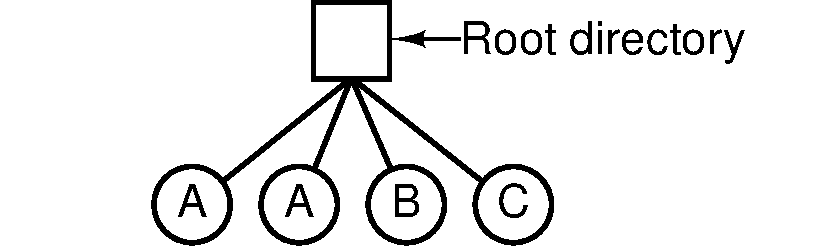
\includegraphics[width=\textwidth]{mos-figs-6-7}
    \end{minipage}\hfill
    \begin{minipage}{.49\textwidth}
      \begin{itemize}
      \item[-] contains 4 files
      \item[-] owned by 3 different people, A, B, and C
      \end{itemize}
    \end{minipage}
  \end{block}
  \begin{block}{Limitations}
    \begin{itemize}
    \item[-] name collision
    \item[-] file searching
    \end{itemize}
  \end{block}
  Often used on simple embedded devices, such as telephone, digital cameras...
\end{frame}

\begin{frame}{Directories}{Two-level Directory Systems}
  \begin{iblock}{A separate directory for each user}
    \begin{center}
      \mode<beamer>{ 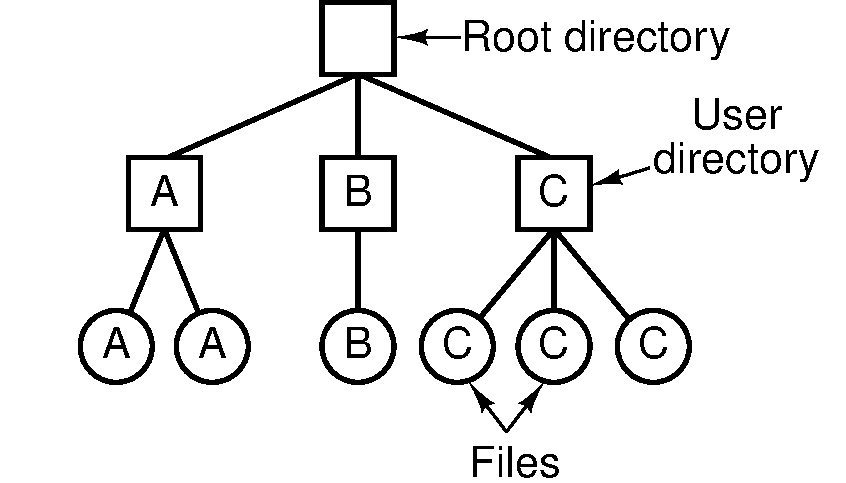
\includegraphics[width=.7\textwidth]{mos-figs-6-8} }%
      \mode<article>{ 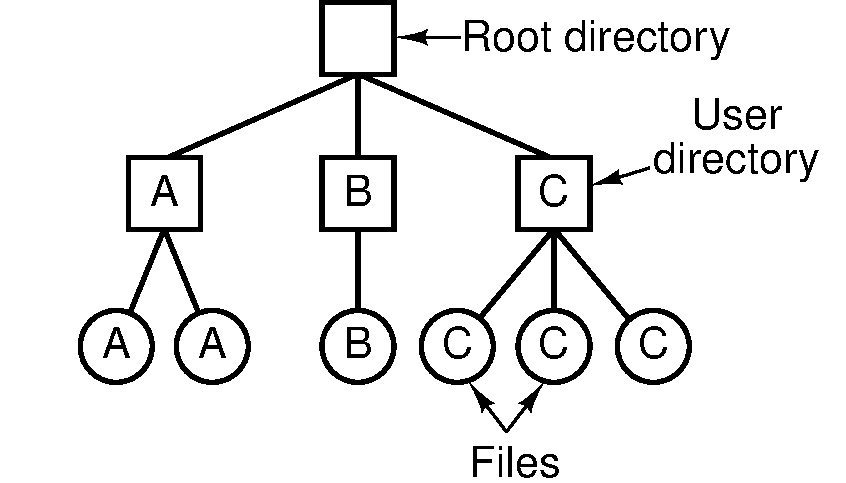
\includegraphics[width=.4\textwidth]{mos-figs-6-8} }
    \end{center}
    \begin{description}
    \item[Limitation:] hard to access others files
    \end{description}
  \end{iblock}
\end{frame}

\begin{frame}{Directories}{Hierarchical Directory Systems}
  \centering
  \mode<beamer>{ 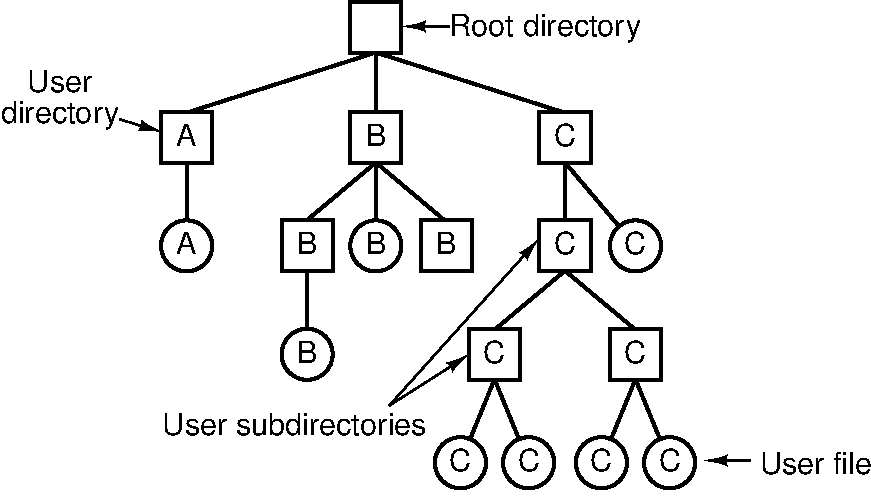
\includegraphics[height=.85\textheight]{mos-figs-6-9} }%
  \mode<article>{ 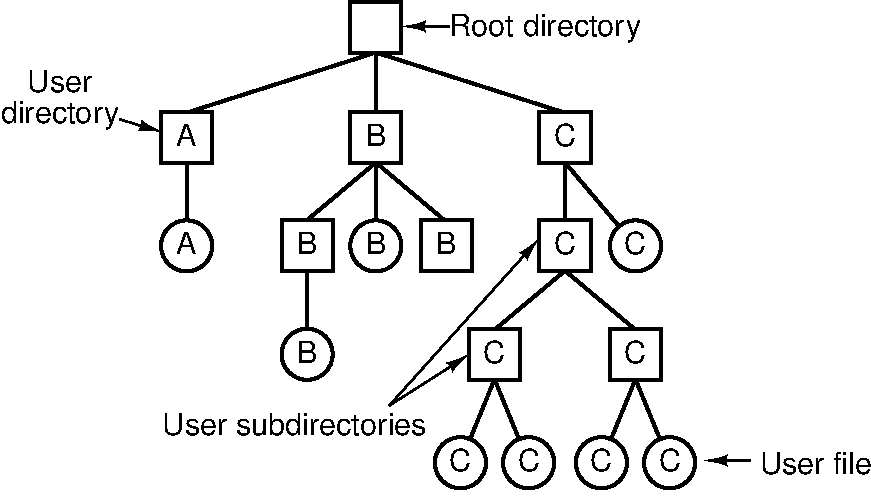
\includegraphics[width=.5\textwidth]{mos-figs-6-9} }
\end{frame}

\begin{frame}{Directories}{Path Names}
  \centering
  \mode<beamer>{ 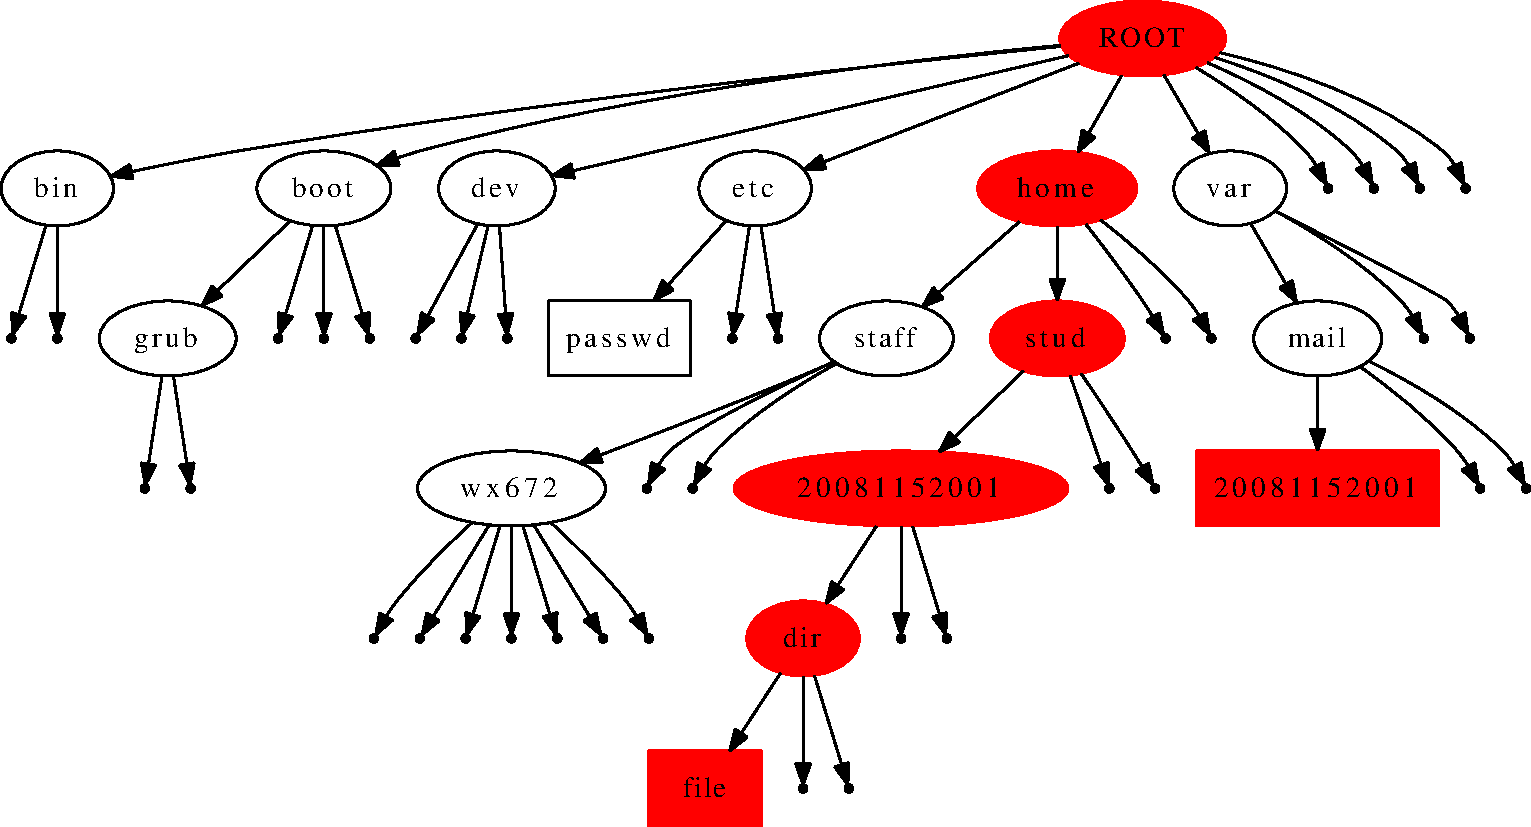
\includegraphics[height=.8\textheight]{cs3} }%
  \mode<article>{ 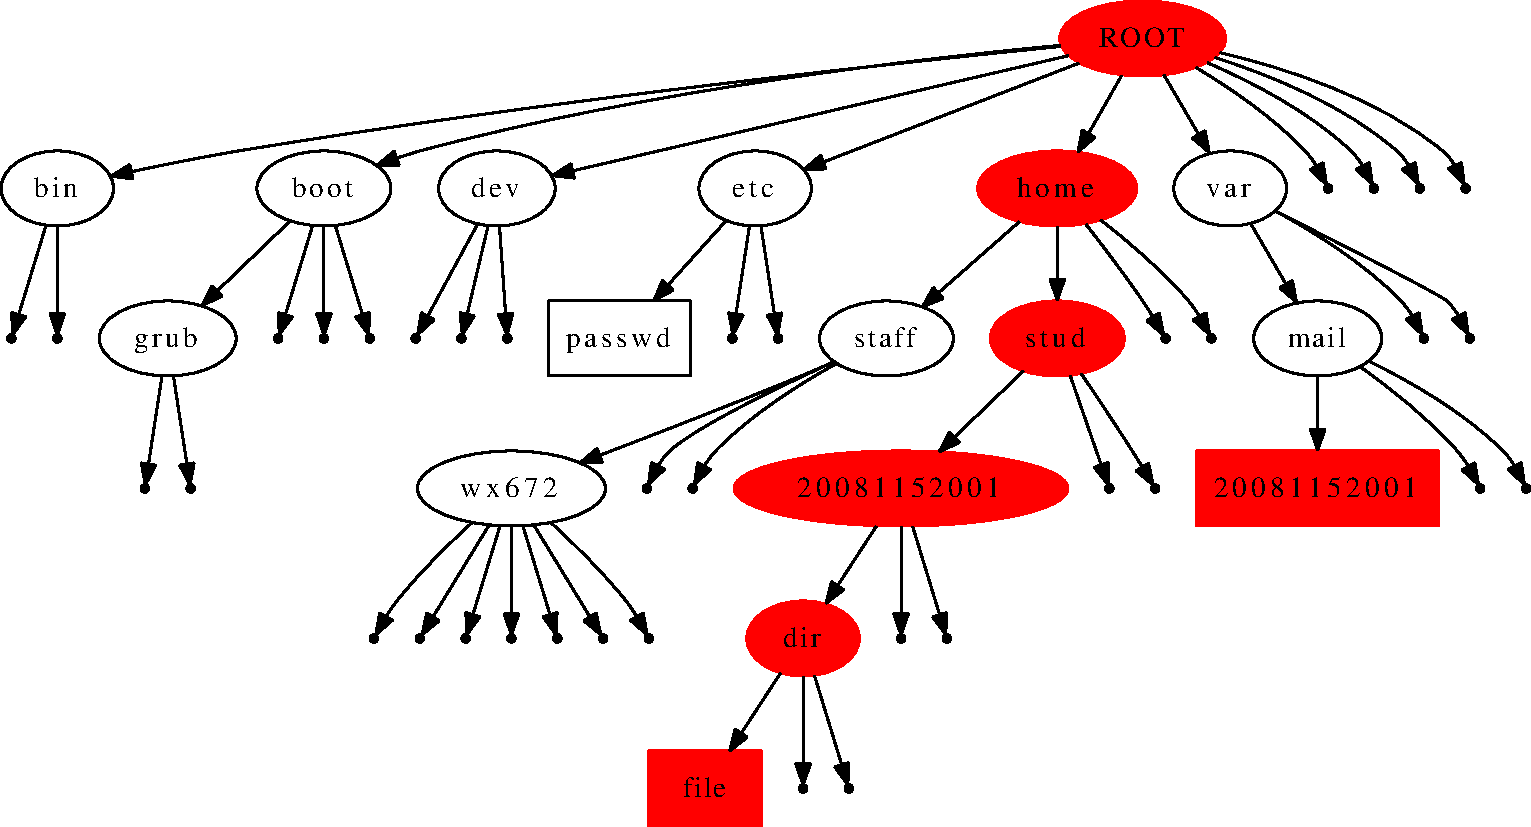
\includegraphics[width=.6\textwidth]{cs3} }
\end{frame}

\begin{frame}{Directories}{Directory Operations}
  \begin{center}
    \begin{tblr}{colspec={llll},rows={font=\ttfamily}}
      opendir()&mkdir()&rename()&link()\\
      closedir()&rmdir()&readdir()&unlink()\\
      \ldots&&&
    \end{tblr}
  \end{center}
\end{frame}

\begin{frame}{\ttfamily ls}
  \mode<beamer>{%
    \begin{tikzpicture}[remember picture, overlay]%
      \node [scale=.3,anchor=east] at (current page.east)%
      {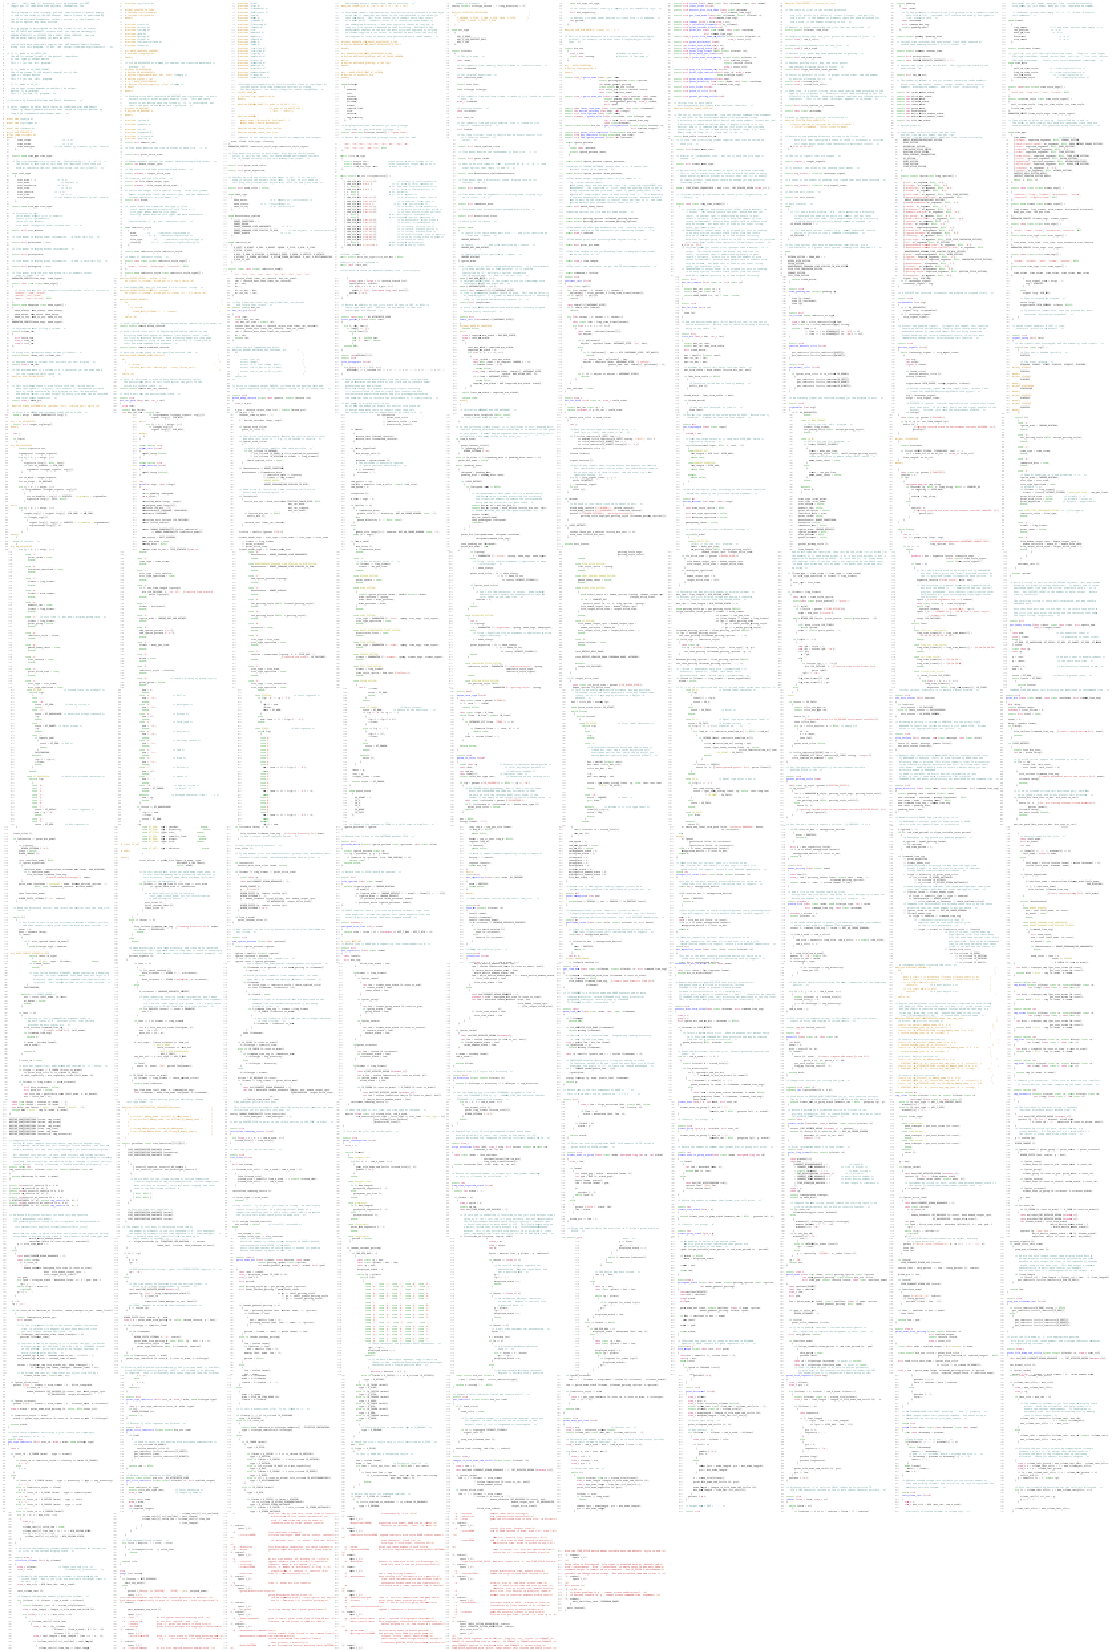
\includegraphics{ls-real}};
    \end{tikzpicture}}
  
  \begin{minipage}{.5\linewidth}
    \mode<beamer>{ \includegraphics[width=\textwidth]{ls-c} }%
    \mode<article>{\cfile{../src/fs/ls.c}}
  \end{minipage}\qquad
  \begin{minipage}{.35\linewidth}
    \begin{description}
    \item[The real \texttt{ls.c}?] 
    \end{description}
    \mode<beamer>{
    \begin{flushright}
      \begin{large}
        116 A4 pages\\
        5308 lines\\[1em]
        Do one thing, and do it really well.\\[2em]
      \end{large}
    \end{flushright}
    {\small \CMD{apt source coreutils}}}
  \mode<article>{
    \begin{itemize}
    \item 116 A4 pages
    \item 5308 lines
    \end{itemize}
    Do one thing, and do it really well.
    \begin{itemize}
    \item[\$] \cmd{apt source coreutils}
    \end{itemize}}
  \end{minipage}
\end{frame}

\begin{frame}{\ttfamily mkdir(), chdir(), rmdir(), getcwd()}
  \centering
  \mode<beamer>{ 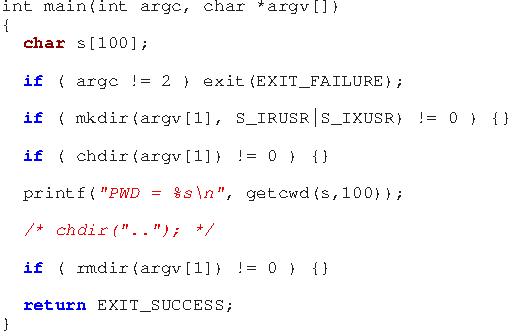
\includegraphics[height=.8\textheight]{mkdir-c} }%
  \mode<article>{\cfile{../src/fs/mkdir.c}}
\end{frame}

\section{File System Implementation}

\subsection{Basic Structures}

\begin{frame}{File System Implementation}
  \begin{block}{A typical file system layout}
    \begin{center}
      \mode<beamer>{ \includegraphics[width=\textwidth]{fs-layout} }%
      \mode<article>{ \includegraphics[width=.5\textwidth]{fs-layout} }
    \end{center}
  \end{block}
  \begin{center}
    \mode<beamer>{ \includegraphics[width=.8\textwidth]{mbr} }%
    \mode<article>{ \includegraphics[width=.5\textwidth]{mbr} }
  \end{center}
\end{frame}

\paragraph{MBR, partition table, and booting}

File systems are stored on disks. Most disks can be divided up into one or more
partitions, with independent file systems on each partition. Sector 0 of the disk is
called the MBR (Master Boot Record ) and is used to boot the computer. The end of the MBR
contains the partition table. This table gives the starting and ending addresses of each
partition. One of the partitions in the table is marked as active. When the computer is
booted, the BIOS reads in and executes the MBR. The first thing the MBR program does is
locate the active partition, read in its first block, called the boot block , and execute
it. The program in the boot block loads the operating system contained in that
partition. For uniformity, every partition starts with a boot block, even if it does not
contain a bootable operating system.  Besides, it might contain one in the future, so
reserving a boot block is a good idea anyway\citetitle[Sec~4.3.1, \emph{File System
  Layout}]{tanenbaum2015modern}.

The \emph{superblock} is read into memory when the computer is booted or the file system
is first touched.

\begin{frame}{On-Disk Information Structure}
  \begin{description}
  \item[Boot control block] a MBR copy
    \begin{itemize}
    \item[UFS:] Boot block
    \item[NTFS:] Partition boot sector
    \end{itemize}
  \item[Volume control block] Contains volume details\par\medskip
      \begin{tblr}{lll}
        number of blocks&free-block count& free FCB count\\
        size of blocks& free-block pointers&free FCB pointers\\
      \end{tblr}
    \begin{itemize}
    \item[UFS:] Superblock
    \item[NTFS:] Master File Table
    \end{itemize}
  \item[Directory structure] Organizes the files \alert{FCB}, \alert{File control block},
    contains file details (metadata).
    \begin{itemize}
    \item[UFS:] I-node
    \item[NTFS:] Stored in MFT using a relational database structure, with one row per
      file
    \end{itemize}
  \end{description}
\end{frame}

\begin{frame}{Each File-System Has a Superblock}
  \begin{block}{Superblock}
    Keeps information about the file system
    \begin{itemize}
    \item Type --- ext2, ext3, ext4...
    \item Size
    \item Status --- how it's mounted, free blocks, free inodes, ...
    \item Information about other metadata structures
    \end{itemize}
  \end{block}
  \begin{itemize}
  \item[\$] \texttt{sudo dumpe2fs /dev/sda1 | less}
  \end{itemize}
\end{frame}

\subsection{Implementing Files}

\begin{frame}{Implementing Files}
  \begin{description}
  \item[Contiguous Allocation] 
  \end{description}
    \begin{center}
      \mode<beamer>{
        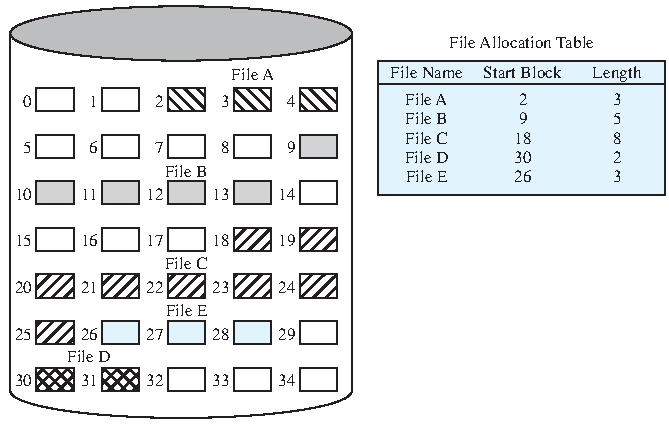
\includegraphics[width=.8\textwidth]{file-alloc-contiguous}
      } \mode<article>{
        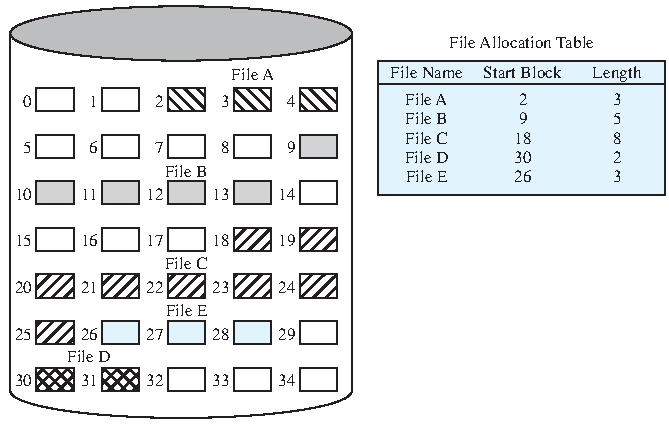
\includegraphics[width=.5\textwidth]{file-alloc-contiguous}
      }
    \end{center}
  \begin{multicols}{2}
    \begin{itemize}
    \item[-] simple;
    \item[-] good for read only;
    \item[-] fragmentation
    \end{itemize}
  \end{multicols}
\end{frame}

\begin{frame}
  \begin{description}
  \item[Linked List (Chained) Allocation] A pointer in each disk block
  \end{description}
  \begin{center}
    \mode<beamer>{ 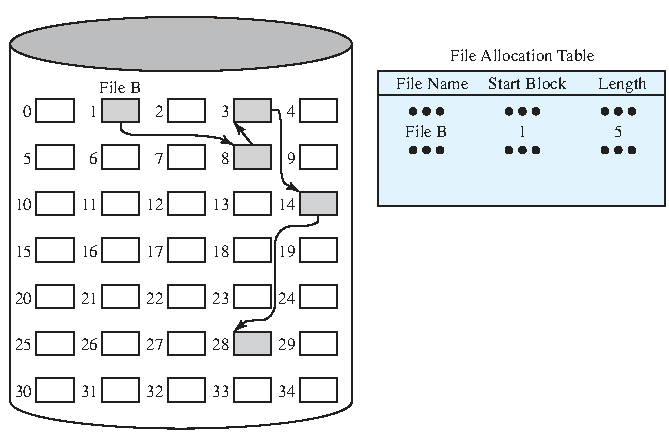
\includegraphics[width=.65\textwidth]{file-alloc-chained} }%
    \mode<article>{ 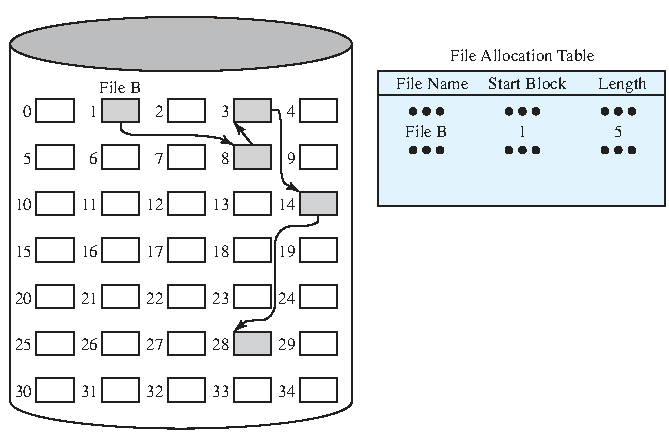
\includegraphics[width=.5\textwidth]{file-alloc-chained} }
  \end{center}
  \begin{multicols}{3}
    \begin{itemize}
    \item[-] no waste block;
    \item[-] slow random access;
    \item[-] not $2^n$
    \end{itemize}
  \end{multicols}
\end{frame}

\paragraph{Consolidation}

One consequence of chaining, as described so far, is that there is \emph{no accommodation
  of the principle of locality}. Thus, if it is necessary to bring in several blocks of a
file at a time, as in sequential processing, then a series of accesses to different parts
of the disk are required. This is perhaps a more significant effect on a single-user
system but may also be of concern on a shared system. To overcome this problem, some
systems periodically consolidate files (fig.  \ref{fig:chained2})\citetitle[Sec.~12.7,
\emph{Secondary Storage Management}, P.~547]{stallings11os}

\begin{frame}
  \begin{description}
  \item[Linked List (Chained) Allocation] Though there is no external fragmentation,
    consolidation is still preferred.
  \end{description}
  \centering
  \mode<beamer>{ 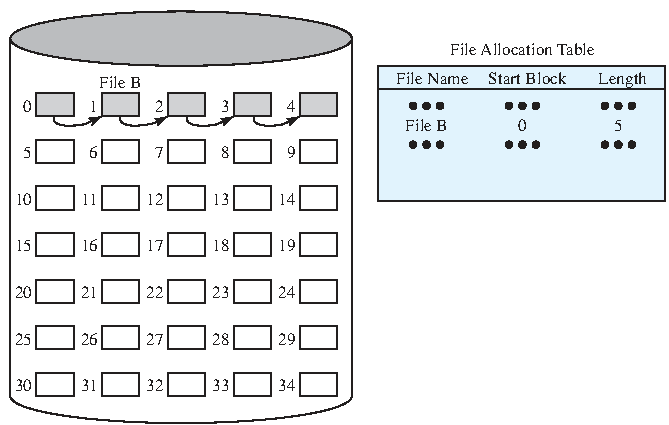
\includegraphics[width=.7\textwidth]{file-alloc-chained2} }%
  \mode<article>{\label{fig:chained2} 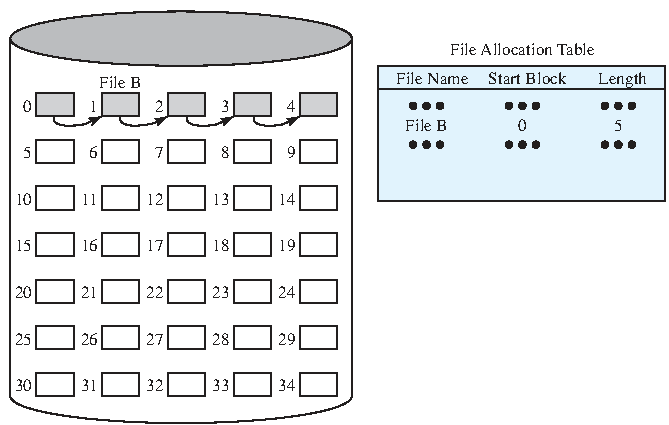
\includegraphics[width=.5\textwidth]{file-alloc-chained2} }
\end{frame}

\begin{frame}
  \begin{itemize}
  \item[FAT:] Linked list allocation with a table in RAM
  \end{itemize}
  \begin{minipage}{.65\textwidth}
    \begin{block}{}
      \begin{itemize}
      \item Taking the pointer out of each disk block, and putting it into a table in
        memory
      \item fast random access (chain is in RAM)
      \item is $2^n$
      \item the entire table must be in RAM
        $$disk\nearrow{}\Rightarrow FAT\nearrow{}\Rightarrow RAM_{used}\nearrow$$
      \end{itemize}
    \end{block}
  \end{minipage}\hfill
  \begin{minipage}{.3\textwidth}
    \centering
    \mode<beamer>{ \includegraphics[width=\textwidth]{fat} }
    \mode<article>{ \includegraphics[width=.8\textwidth]{fat} }
  \end{minipage}
\end{frame}

See also: \citetitle[\emph{Wikipedia:FAT}]{wiki:fat}.

\begin{frame}
  \begin{iblock}{Indexed Allocation}
    \centering%
    \mode<beamer>{ 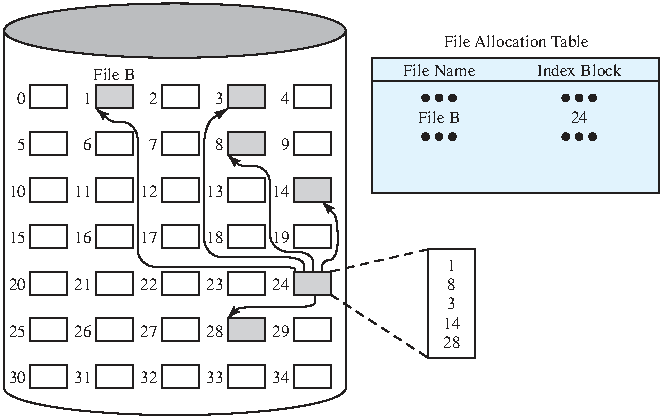
\includegraphics[width=.7\textwidth]{file-alloc-idx} }%
    \mode<article>{ 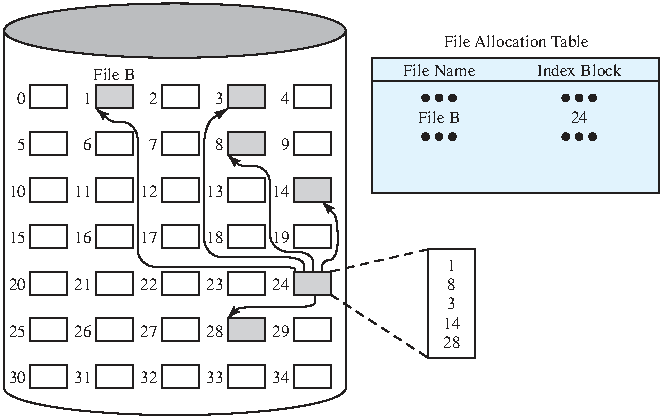
\includegraphics[width=.4\textwidth]{file-alloc-idx} }    
  \end{iblock}
  \begin{description}
  \item[I-node] A data structure for each file. An i-node is in memory \emph{only if} the
    file is open
    $$files_{opened}\nearrow{}\Rightarrow{}RAM_{used}\nearrow{}$$
  \end{description}
\end{frame}

See also: \citetitle[\emph{Wikipedia:inode}]{wiki:inode}.

\begin{frame}{I-node --- FCB in UNIX}
  \begin{minipage}[t]{.4\textwidth}
    \centering
    \mode<beamer>{ 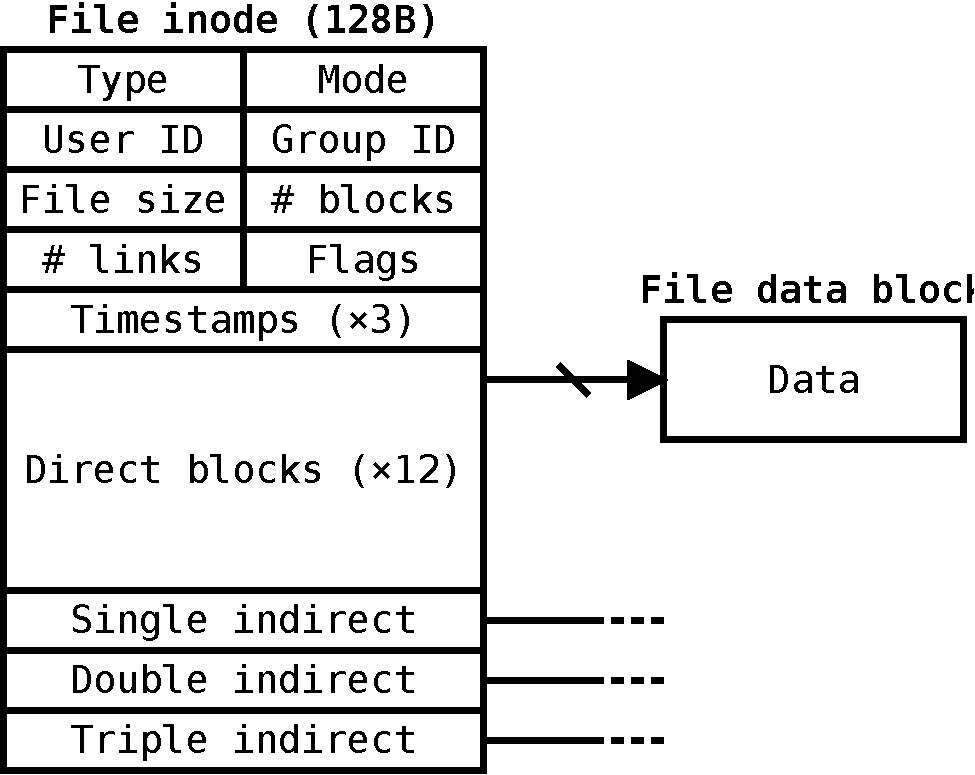
\includegraphics[width=1.4\textwidth]{inode-struct2} }%
    \mode<article>{ 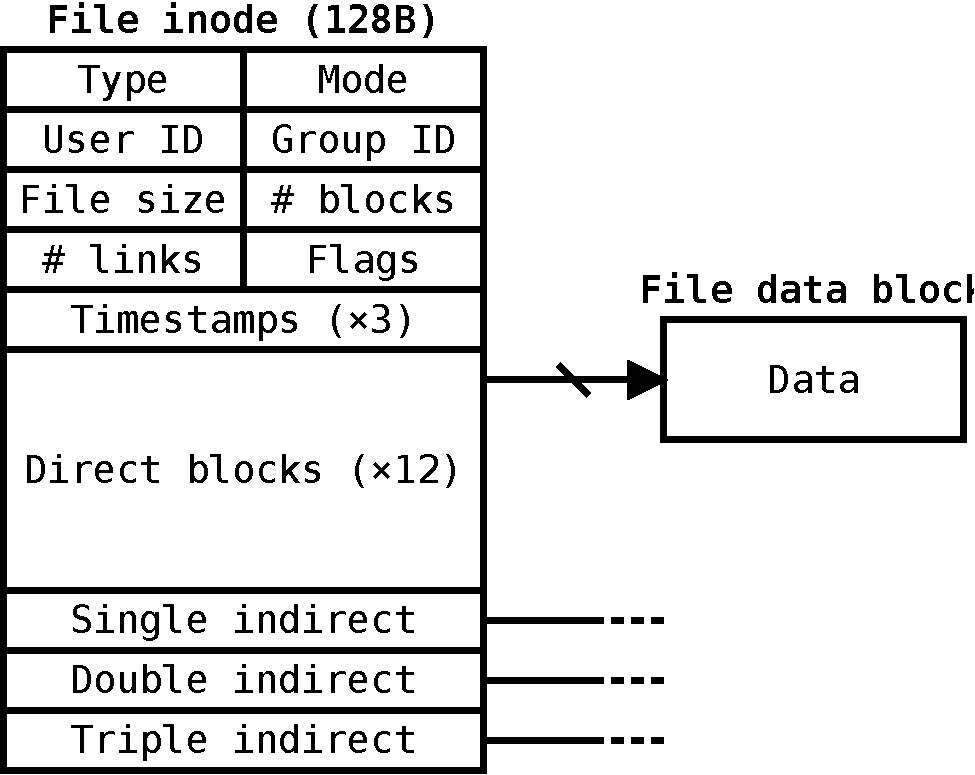
\includegraphics[width=.7\textwidth]{inode-struct2} }
  \end{minipage}\hfill
  \begin{minipage}[b]{.45\textwidth}
    \centering
    \begin{tblr}{colspec={cl},hline{1,2,Z},row{1}={font=\bfseries}}
      File type&Description\\
      0&Unknown\\
      1&Regular file\\
      2&Directory\\
      3&Character device\\
      4&Block device\\
      5&Named pipe\\
      6&Socket\\
      7&Symbolic link\\
    \end{tblr}
    \vspace{1em}
    \begin{description}
    \item[Mode:] 9-bit pattern
    \end{description}
  \end{minipage}
\end{frame}

\paragraph{A little quiz}

\begin{itemize}
\item in one terminal, to create a file ``a'', do:
  \begin{itemize}
  \item[\$] \texttt{echo hello > /tmp/a} 
  \end{itemize}
\item to track its contents and keep it open, do:
  \begin{itemize}
  \item[\$] \texttt{tail -f /tmp/a}
  \end{itemize}
\item in another terminal, delete this file ``a'', do:
  \begin{itemize}
  \item[\$] \texttt{rm -f /tmp/a}
  \end{itemize}
\item make sure it's gone, do:
  \begin{itemize}
  \item[\$] \texttt{ls -l /tmp/a}
  \item[\$] \texttt{ls -li /proc/`pidof tail`/fd}
  \item[\$] \texttt{lsof -p `pidof tail` | grep deleted}
  \end{itemize}
  as you can see, \texttt{/tmp/a} is marked as ``deleted''. Now, do:
  \begin{itemize}
  \item[\$] \texttt{echo "another a" >> /tmp/a}
  \item[\$] \texttt{ls -li /tmp/a}
  \end{itemize}
  Is this \texttt{/tmp/a} same as the deleted one? (check the inodes)
\end{itemize}

\begin{frame}{Inode Quiz}
  \begin{description}
  \item[Given:] block size is 1KB; pointer size is 4B
  \item[Addressing:] byte offset 9000; byte offset 350,000
  \end{description}
  \centering
  \mode<beamer>{ \includegraphics[width=.65\textwidth]{inode-calc2} }%
  \mode<article>{ \includegraphics[width=.5\textwidth]{inode-calc2} }
\end{frame}

Several block entries in the inode are 0, meaning that the logical block entries contain
no data. This happens if no process ever wrote data into the file at any byte offsets
corresponding to those blocks and hence the block numbers remain at their initial value,
0. No disk space is wasted for such blocks. Process can cause such a block layout in a
file by using the \verb|lseek()| and \verb|write()| system calls\citetitle[Sec.~4.2,
\emph{Structure of a Regular File}]{bach1986design}.

\begin{frame}{UNIX In-Core Data Structure}
  \begin{description}
  \item[mount table] --- Info about each mounted FS
  \item[directory-structure cache] --- Dir-info of recently
      accessed dirs
  \item[inode table] --- An in-core version of the on-disk inode table
  \item[file table]\ 
    \begin{itemize}
    \item global
    \item keeps inode of each open file
    \item keeps track of
      \begin{itemize}
      \item how many processes are associated with each open file
      \item where the next read and write will start
      \item access rights
      \end{itemize}
    \end{itemize}
  \item[user file descriptor table]\ 
    \begin{itemize}
    \item per process
    \item identifies all open files for a process
    \end{itemize}
  \end{description}
\end{frame}

Find them in the kernel source
  \begin{description}
  \item[user file descriptor table] --- \texttt{struct fdtable} in
    \texttt{include/linux/fdtable.h}
  \item[open file table] --- \texttt{struct files\_struct} in
    \texttt{include/linux/fdtable.h}
  \item[inode] --- \texttt{struct inode} in \texttt{include/linux/fs.h}
  \item[inode table] --- ?
  \item[superblock] --- \texttt{struct super\_block} in \texttt{include/linux/fs.h}
  \item[dentry] --- \texttt{struct dentry} in \texttt{include/linux/dcache.h}
  \item[file] --- \texttt{struct file} in \texttt{include/linux/fs.h}
  \end{description}

\begin{frame}{UNIX In-Core Data Structure}
  \centering
  \mode<beamer>{ \includegraphics[width=.5\textwidth]{fs-tables} }
  \mode<article>{ \includegraphics[width=.4\textwidth]{fs-tables}\label{fig:tables} }
  \begin{block}{\texttt{open()}/\texttt{creat()}}
    \begin{enumerate}
    \item add entry in each table
    \item returns a \alert{file descriptor} --- an index into the user file descriptor table
    \end{enumerate}
  \end{block}
\end{frame}

\paragraph{Open file descriptor table}

a global table, whose address is contained in the \texttt{files} field of the process
descriptor, specifies which files are currently opened by the process. It is a
\texttt{files\_struct} structure whose fields are illustrated in
Table~\ref{tbl:filestruct}\citetitle[Sec.~12.2.6, \emph{Files Associated with a
  Process}]{bovet2005understanding}.

\begin{table}[!h]
  \centering
  \caption{The fields of the \texttt{files\_struct} structure}
  \label{tbl:filestruct}% this line have to follow \caption
  \begin{tblr}{width=\textwidth,colspec={llX},row{1}={font=\bfseries},
      column{1,2}={font=\ttfamily},hline{1,2,Z}}
    Type   &Field&Description\\
    atomic\_t       &count&Number of processes sharing this table\\
    rwlock\_t       &file\_lock&Read/write spin lock for the table fields\\
    int             &max\_fds&Current maximum number of file objects\\
    int             &max\_fdset&Current maximum number of file descriptors\\
    int             &next\_fd&Maximum file descriptors ever allocated plus 1\\
    struct file **  &fd&Pointer to array of file object pointers\\
    fd\_set *       &close\_on\_exec&Pointer to file descriptors to be closed on \texttt{exec()}\\
    fd\_set *       &open\_fds&Pointer to open file descriptors\\
    fd\_set         &close\_on\_exec\_init&Initial set of file descriptors to be closed on \texttt{exec()}\\
    fd\_set         &open\_fds\_init&Initial set of file descriptors\\
    struct file *[] &fd\_array&Initial array of file object pointers\\
  \end{tblr}
\end{table}
  
The \texttt{fd} field points to an array of pointers to file objects. The size of the
array is stored in the \texttt{max\_fds} field. Usually, \texttt{fd} points to the
\texttt{fd\_array} field of the \texttt{files\_struct} structure, which includes 32 file
object pointers. If the process opens more than 32 files, the kernel allocates a new,
larger array of file pointers and stores its address in the \texttt{fd} fields; it also
updates the \texttt{max\_fds} field.

For every file with an entry in the \texttt{fd} array, the array index is the file
descriptor. Usually, the first element (index 0) of the array is associated with the
standard input of the process, the second with the standard output, and the third with the
standard error (See fig.~12-3\footnote{In book Understanding The Linux Kernel}). Unix
processes use the file descriptor as the main file identifier. Notice that, thanks to the
\verb|dup()| , \verb|dup2()| , and \verb|fcntl()| system calls, two file descriptors may
refer to the same opened file, that is, two elements of the array could point to the same
file object. Users see this all the time when they use shell constructs such as
\texttt{2>\&1} to redirect the standard error to the standard output.

\paragraph{\texttt{open()}}

A call to \verb|open()| creates a new \emph{open file description}, an entry in the
system-wide table of open files.  This entry records the file offset and the file status
flags (modifiable via the \texttt{fcntl(2)} \verb|F_SETFL| operation). \emph{A file
  descriptor is a reference to one of these entries; this reference is unaffected if
  \texttt{pathname} is subsequently removed or modified to refer to a different file.  The
  new \emph{open file description} is initially not shared with any other process, but
  sharing may arise via \texttt{fork(2)} [\texttt{man 2 open}].}
  
The internal representation of a file is given by an \emph{inode}, which contains a
description of the disk layout of the file data and other information such as the file
owner, access permissions, and access times. The term inode is a contraction of the term
index node and is commonly used in literature on the UNIX system. Every file has one
inode, but it may have several names, all of which map into the inode. Each name is called
a \emph{link}.  When a process refers to a file by name, the kernel parses the file name
one component at a time, checks that the process has permission to search the directories
in the path, and eventually retrieves the inode for the file. For example, if a process
calls

\mint{c}|  open("/fs2/mjb/rje/sourcefile",1);|

the kernel retrieves the inode for ``\verb|/fs2/mjb/rje/sourcefile|''. When a process
creates a new file, the kernel assigns it an unused inode. Inodes are stored in the file
system, as will be seen shortly, but the kernel reads them into an in-core inode table
when manipulating files.

The kernel contains two other data structures, the \emph{file table} and the \emph{user
  file descriptor table}. The file table is a global kernel structure, but the user file
descriptor table is allocated per process. When a process \texttt{open}s or
\texttt{creat}s a file, the kernel allocates an entry from each table, corresponding to
the file's inode. \emph{Entries in the three structures --- user file descriptor table,
  file table, and inode table --- maintain the state of the file and the user's access to
  it.} The file table keeps track of the byte offset in the file where the user's next
\texttt{read} or \texttt{write} will start, and the access rights allowed to the
\texttt{open}ing process. The user file descriptor table identifies all open files for a
process.  Fig.~\ref{fig:tables} shows the tables and their relationship to each other. The
kernel returns a \emph{file descriptor} for the \texttt{open} and \texttt{creat} system
calls, which is an index into the user file descriptor table. When executing \texttt{read}
and \texttt{write} system calls, the kernel uses the file descriptor to access the user
fie descriptor table, follows pointers to the file table and inode table entries, and,
from the inode, finds the data in the file. Chapters 4 and 5 describe these data
structures in great detail. For now, suffice it to say that use of three tables allows
various degrees of sharing access to a file\citetitle[Sec.~2.2.1, \emph{An Overview of the
  File Subsystem}]{bach1986design}.

The \texttt{open} system call is the first step a process must take to access the data in
a file. The syntax for the \texttt{open} system call is

\mint{c}|  fd = open(pathname, flags, modes);|

where \emph{pathname} is a file name, \emph{flags} indicate the type of open (such as for
reading or writing), and \emph{modes} give the file permissions if the file is being
created. The \texttt{open} system call returns an integer called the user \emph{file
  descriptor}. Other file operations, such as reading, writing, seeking, duplicating the
file descriptor, setting file I/O parameters, determining file status, and closing the
file, use the file descriptor that the \texttt{open} system call returns\citetitle[Sec.~5.1,
\emph{Open}]{bach1986design}.

The kernel searches the file system for the file name parameter using algorithm
\emph{namei} (see fig.~\ref{fig:open}). It checks permissions for opening the file after
it finds the in-core inode and allocates an entry in the file table for the open file. The
file table entry contains a pointer to the inode of the open file and a field that
indicates the byte offset in the file where the kernel expects the next \texttt{read} or
\texttt{write} to begin. The kernel initializes the offset to 0 during the \texttt{open}
call, meaning that the initial \texttt{read} or \texttt{write} starts at the beginning of
a file by default. Alternatively, a process can \texttt{open} a file in
\emph{write-append} mode, in which case the kernel initializes the offset to the size of
the file. The kernel allocates an entry in a private table in the process \emph{u area},
called the user file descriptor table, and notes the index of this entry. The index is the
file descriptor that is returned to the user. The entry in the user file table points to
the entry in the global file table.

\begin{figure}[h]
  \centering
  \begin{minipage}[h]{.8\linewidth}
\begin{verbatim}
algorithm open
inputs: file name
        type of open
        file permissions (for creation type of open)
output: file descriptor
{
   convert file name to inode (algorithm namei);
   if (file does not exist or not permitted access)
           return (error);
   allocate file table entry for inode, initialize count, offset;
   allocate user file descriptor entry, set pointer to file table entry;
   if (type of open specifies truncate file)
          free all file blocks (algorithm free);
   unlock (inode); /* locked above in namei */
   return (user file descriptor);
}
\end{verbatim}
  \end{minipage}
  \caption{Algorithm for opening a file}
  \label{fig:open}
\end{figure}

\begin{description}
\item[Q1:] Can \texttt{open()} return an inode number?
\item[Q2:] Can we keep the I/O pointers in the inode? Possibly adding a few pointers in
  the inode data structure in a similar fashion of those block pointers
  (direct/single-indirect/double-indirect/triple-indirect). Each pointer pointing to an
  I/O pointer record. 
\end{description}
% \begin{frame} !!! Probably wrong !!!
%   \begin{block}{When \texttt{open(pathname,flags)} is called,}
%     \begin{enumerate}
%     \item the directory structure is searched for the given file name
%     \item retrieves the \emph{ID} for the file
%     \item search system-wide open-file table
%       \begin{itemize}
%       \item[if] the file is opened already by another process
%       \item[then] create an entry in per-process table
%         \begin{itemize}
%         \item[] pointing to the entry in sys-wide open-file table
%         \end{itemize}
%       \item[else] create an entry in sys-wide open-file table, and
%         \begin{itemize}
%         \item[] create an entry in per-process table pointing to the entry in sys-wide
%           table
%         \end{itemize}
%       \end{itemize}
%     \end{enumerate}
%   \end{block}
% \end{frame}

\begin{frame}{The Tables}%{A File Is Opened By Multiple Processes?}
  \begin{block}{Two levels of internal tables in the OS}
    \begin{description}
      \item[A per-process table] tracks all files that a process has open. Stores
        \begin{itemize}
        \item the current-file-position pointer (not really)
        \item access rights
        \item more...
        \end{itemize}
        a.k.a file descriptor table
      \item[A system-wide table] keeps process-independent information, such as
        \begin{itemize}
        \item the location of the file on disk
        \item access dates
        \item file size
        \item file open count --- the number of processes opening this file
        \end{itemize}
    \end{description}    
  \end{block}  
\end{frame}

\begin{frame}<article>%{What If A File Opened By Multiple Processes?}
  \begin{center}
    \mode<beamer>{ 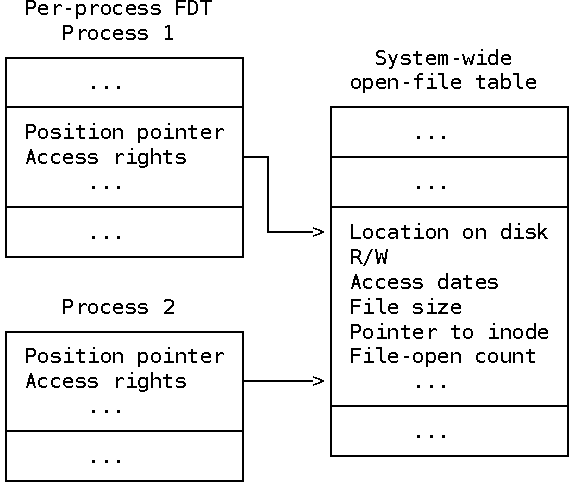
\includegraphics[width=.8\textwidth]{file-tables} }%
    \mode<article>{ 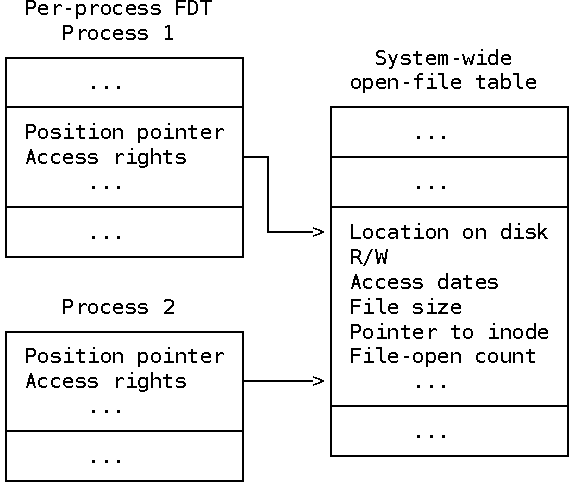
\includegraphics[width=.5\textwidth]{file-tables} }
  \end{center}
\end{frame}

\begin{frame}
  \begin{block}{A process executes the following code:}
    \begin{itemize}
    \item[] \texttt{fd1 = open("/etc/passwd", O\_RDONLY);}
    \item[] \texttt{fd2 = open("local", O\_RDWR);}
    \item[] \texttt{fd3 = open("/etc/passwd", O\_WRONLY);}
    \end{itemize}
  \end{block}
  \centering
  \mode<beamer>{ 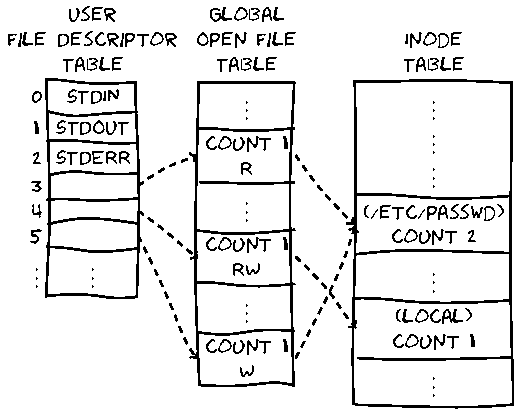
\includegraphics[width=.5\textwidth]{file-tables2} }%
  \mode<article>{ 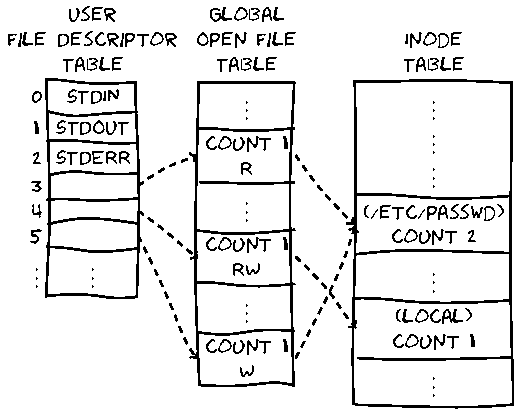
\includegraphics[width=.6\textwidth]{file-tables2} }
\end{frame}

See also:
\begin{itemize}
\item \citetitle[Sec.~5.1, \emph{Open}]{bach1986design}.
\item File descriptor
  manipulation\footnote{\url{http://www.cim.mcgill.ca/~franco/OpSys-304-427/lecture-notes/node27.html\#SECTION00063000000000000000}}.
\end{itemize}

\begin{frame}
  \begin{block}{One more process B:}
    \begin{itemize}
    \item[] \texttt{fd1 = open("/etc/passwd", O\_RDONLY);}
    \item[] \texttt{fd2 = open("private", O\_RDONLY);}
    \end{itemize}
  \end{block}
  \centering
  \mode<beamer>{ 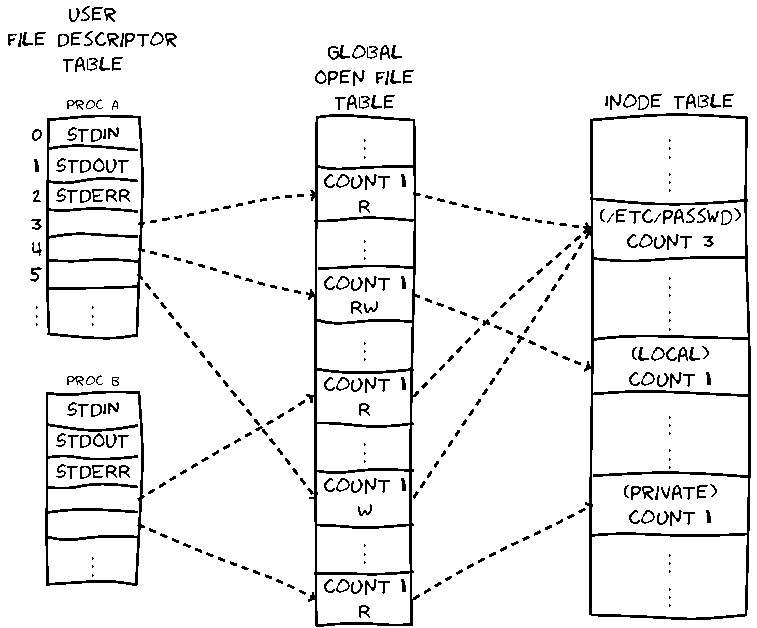
\includegraphics[width=.5\textwidth]{file-tables3} }%
  \mode<article>{ 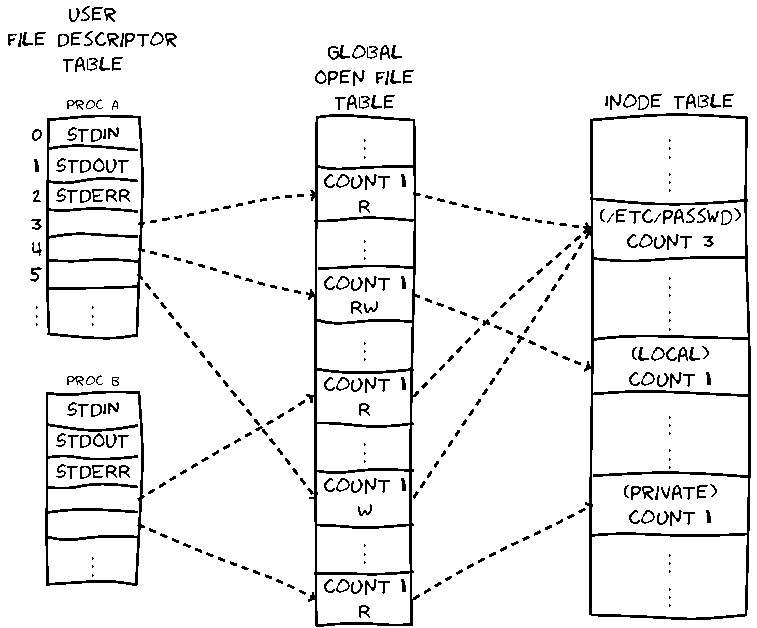
\includegraphics[width=.6\textwidth]{file-tables3} }
\end{frame}

\begin{frame}{Why File Table?}
  To allow a parent and child to share a file position, but to provide unrelated processes
  with their own values.
  
  \label{fig:filetable}
  \centering
  \mode<beamer>{ 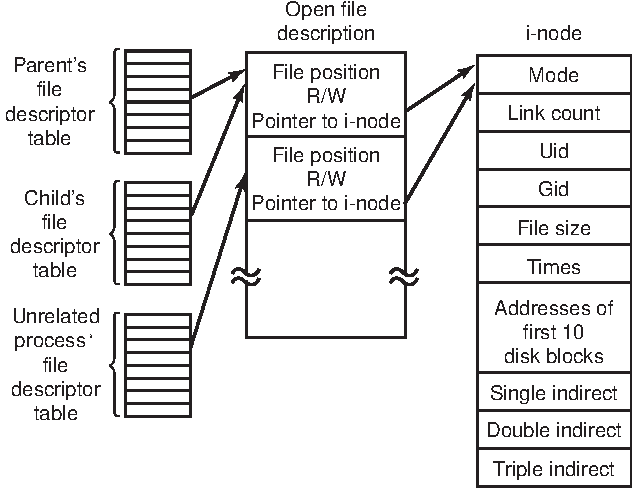
\includegraphics[width=.6\textwidth]{mos-10-33} }%
  \mode<article>{ 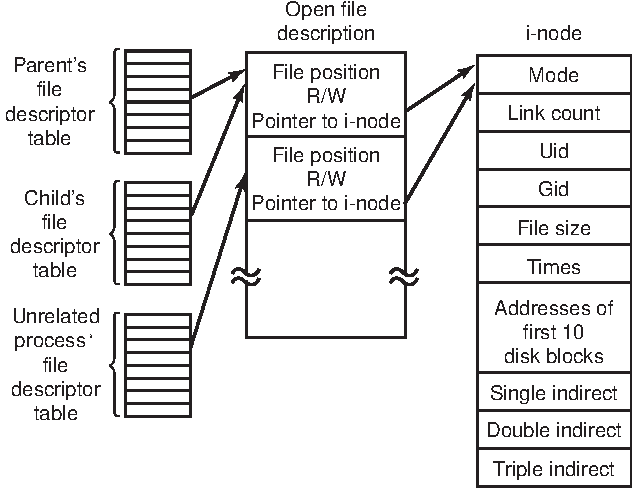
\includegraphics[width=.5\textwidth]{mos-10-33} }
\end{frame}

\begin{frame}{Why File Table?}
  \begin{block}{Where To Put File Position Info?}
    \begin{description}
    \item[Inode table?] No. Multiple processes can open the same file. Each one has its
      own file position.
    \item[User file descriptor table?] No. Trouble in file sharing.
    \end{description}
  \end{block}
  \begin{block}{Example}
    \begin{minipage}{.22\textwidth}
      \begin{center}
        \mode<beamer>{ \includegraphics[width=\textwidth]{fs-hello-sh} }%
        \mode<article>{ \shellfile{figs/pseudo/fs-hello.sh} }
      \end{center}
    \end{minipage}\qquad
    \begin{minipage}{.7\textwidth}
      \begin{itemize}
        \item[\$] \texttt{./hello.sh > A}
        \item[?] Where should the ``\texttt{world}'' be?
      \end{itemize}
    \end{minipage}
  \end{block}
\end{frame}

Why file table?
\begin{description}
\item[File system implementation] With file sharing, it is necessary to allow related
  processes to share a common I/O pointer and yet have separate I/O pointers for
  independent processes that access the same file.  With these two conditions, the I/O
  pointer cannot reside in the i-node table nor can it reside in the list of open files for
  the process.  A new table (the open file table) was invented for the sole purpose of
  holding the I/O pointer. Processes that share the same open file (the result of
  \texttt{fork}s) share a common open file table entry.  A separate open of the same file
  will only share the i-node table entry, but will have distinct open file table
  entries\citetitle[Sec.~4.1]{thompson78uniximplementation}.
\item[Open] The user file descriptor table entry could conceivably contain the file offset
  for the position of the next I/O operation and point directly to the in-core inode entry
  for the file, eliminating the need for a separate kernel file table. The examples above
  show a one-to-one relationship between user file descriptor entries and kernel file
  table entries. Thompson notes, however, that he implemented the file table as a separate
  structure to allow sharing of the offset pointer between several user file
  descriptors\citetitle[\emph{Thompson~78, p.~1943}]{thompson78uniximplementation}. The
  \texttt{dup} and \texttt{fork} system calls, explained in
  \citetitle[Sec.~5.13]{bach1986design} and \citetitle[Sec.~7.1]{bach1986design},
  manipulate the data structures to allow such sharing
  \citetitle[Sec.~5.1]{bach1986design}.
\item[The Linux File System] ... The idea is to start with this file descriptor and end up
  with the corresponding i-node. Let us consider one possible design: just put a pointer
  to the i-node in the file descriptor table. Although simple, unfortunately this method
  does not work.  The problem is as follows. Associated with every file descriptor is a
  file position that tells at which byte the next read (or write) will start. Where should
  it go?  One possibility is to put it in the i-node table. However, this approach fails
  if two or more unrelated processes happen to open the same file at the same time because
  each one has its own file position\citetitle[Sec.~10.6]{tanenbaum2015modern}.

  A second possibility is to put the file position in the file descriptor table. In that
  way, every process that opens a file gets its own private file position. Unfortunately
  this scheme fails too, but the reasoning is more subtle and has to do with the nature of
  file sharing in Linux. Consider a shell script, \texttt{s}, consisting of two commands,
  \texttt{p1} and \texttt{p2}, to be run in order. If the shell script is called by the
  command line

  \texttt{S >X}

  it is expected that \texttt{p1} will write its output to \texttt{x}, and then
  \texttt{p2} will write its output to \texttt{x} also, starting at the place where
  \texttt{p1} stopped.

  When the shell forks off \texttt{p1}, \texttt{x} is initially empty, so \texttt{p1} just
  starts writing at file position 0. However, when \texttt{p1} finishes, some mechanism is
  needed to make sure that the initial file position that \texttt{p2} sees is not 0 (which
  it would be if the file position were kept in the file descriptor table), but the value
  \texttt{p1} ended with.

  The way this is achieved is shown in Fig~\ref{fig:filetable}. The trick is to introduce
  a new table, the \emph{open file description table}, between the file descriptor table
  and the i-node table, and put the file position (and read/write bit) there. In this
  figure, the parent is the shell and the child is first \texttt{p1} and later
  \texttt{p2}. When the shell forks off \texttt{p1}, its user structure (including the
  file descriptor table) is an exact copy of the shell's, so both of them point to the
  same open file description table entry. When \texttt{p1} finishes, the shell's file
  descriptor is still pointing to the open file description containing p1's file
  position. When the shell now forks off \texttt{p2}, the new child automatically inherits
  the file position, without either it or the shell even having to know what that position
  is.
\end{description}

\subsection{Implementing Directories}

\begin{frame}{Implementing Directories}
  \begin{center}\label{fig:dir}
    \mode<beamer>{ \includegraphics[width=\textwidth]{mos-figs-6-16} }%
    \mode<article>{ \includegraphics[width=.5\textwidth]{mos-figs-6-16} }
  \end{center}
  \begin{itemize}
  \item[(a)] A simple directory (Windows)
    \begin{itemize}
    \item fixed size entries
    \item disk addresses and attributes in directory entry
    \end{itemize}
  \item[(b)] Directory in which each entry just refers to an i-node (UNIX)
  \end{itemize}
\end{frame}

The maximum possible size for a file on a FAT32 volume is 4 GiB minus 1 byte or
4,294,967,295 ($2^{32} − 1$) bytes. This limit is a consequence of the file length entry
in the directory table and would also affect huge FAT16 partitions with a sufficient
sector size\citetitle{wiki:fat}.

\begin{frame}%{Directory}
  \begin{block}{Directory entry in \texttt{glibc}}
    \mode<beamer>{ \includegraphics[width=\textwidth]{dirent-c} }%
    \mode<article>{\cfile{../src/fs/dirent.c}}
  \end{block}
  \begin{itemize}
  \item[\$] \cmd{man readdir}
  \item[\$] \cmd{view /usr/include/x86\_64-linux-gnu/bits/dirent.h}
  \end{itemize}
\end{frame}

\begin{frame}{How Long A File Name Can Be?}
  \label{fig:filename}
  \centering
  \mode<beamer>{ \includegraphics[width=.75\textwidth]{dir1} }%
  \mode<article>{ \includegraphics[width=.5\textwidth]{dir1} }
\end{frame}

How long file name is implemented?
\begin{enumerate}
\item The simplest approach is to set a limit on file name length, typically 255
  characters, and then use one of the designs of fig.~\ref{fig:dir} with 255 characters
  reserved for each file name. This approach is simple, but wastes a great deal of
  directory space, since few files have such long names. For efficiency reasons, a
  different structure is desirable.
\item One alternative is to give up the idea that all directory entries are the same
  size. With this method, each directory entry contains a fixed portion, typically
  starting with the length of the entry, and then followed by data with a fixed format,
  usually including the owner, creation time, protection information, and other
  attributes. This fixed-length header is followed by the actual file name, however long
  it may be, as shown in fig.~\ref{fig:filename}(a) in big-endian format (e.g., SPARC). In
  this example we have three files, project-budget, personnel, and foo. Each file name is
  terminated by a special character (usually 0), which is represented in the figure by a
  box with a cross in it. To allow each directory entry to begin on a word boundary, each
  file name is filled out to an integral number of words, shown by shaded boxes in the
  figure.

  A disadvantage of this method is that when a file is removed, a variable-sized gap is
  introduced into the directory into which the next file to be entered may not fit. This
  problem is the same one we saw with contiguous disk files, only now compacting the
  directory is feasible because it is entirely in memory. Another problem is that a single
  directory entry may span multiple pages, so a page fault may occur while reading a file
  name.
\item Another way to handle variable-length names is to make the directory entries
  themselves all fixed length and keep the file names together in a heap at the end of the
  directory, as shown in fig.~\ref{fig:filename}(b). This method has the advantage that
  when an entry is removed, the next file entered will always fit there. Of course, the
  heap must be managed and page faults can still occur while processing file names. One
  minor win here is that there is no longer any real need for file names to begin at word
  boundaries, so no filler characters are needed after file names in
  fig.~\ref{fig:filename}(b) as they are in fig.~\ref{fig:filename}(a).
\item Ext2's approach is a bit different. See Sec.~\ref{sec:ext2-directory}.
\end{enumerate}
See also: \citetitle[Sec.~4.3.3, \emph{Implementating Directories}]{tanenbaum2015modern}.

\begin{frame}{UNIX Treats a Directory as a File}
  \mode<beamer>{\centering \includegraphics[height=.9\textheight]{inode-struct}}%
  \mode<article>{\includegraphics[width=.6\textwidth]{inode-struct}}
\end{frame}

\begin{itemize}
\item A directory is a file whose data is a sequence of entries, each consisting of an
  inode number and the name of a file contained in the directory.
\item Each (disk) block in a directory file consists of a linked list of entries; each
  entry contains the length of the entry, the name of a file, and the inode number of the
  inode to which that entry refers\citetitle[Sec.~15.7.2, \emph{The Linux ext2fs File
    System}]{silberschatz13essentials}.
\end{itemize}

\begin{frame}
  \begin{iblock}{The steps in looking up \texttt{/usr/ast/mbox}}
    \begin{center}\label{fig:dir-lookup}
      \mode<beamer>{ \includegraphics[width=.9\textwidth]{dir-traverse} }%
      \mode<article>{ \includegraphics[width=.5\textwidth]{dir-traverse} }
    \end{center}
  \end{iblock}
\end{frame}

\begin{itemize}
\item First the file system locates the root directory.  In UNIX its i-node is located at
  a fixed place on the disk. From this i-node, it locates the root directory, which can be
  anywhere on the disk, but say block \texttt{1}\citetitle[Sec.~4.5, \emph{Example File
    Systems}]{tanenbaum2015modern}.

  Then it reads the root directory and looks up the first component of the path,
  \texttt{usr}, in the root directory to find the i-node number of the file
  \texttt{/usr}. Locating an i-node from its number is straightforward, since each one has a
  fixed location on the disk. From this i-node, the system locates the directory for
  \texttt{/usr} and looks up the next component, \texttt{ast}, in it. When it has found the
  entry for \texttt{ast}, it has the i-node for the directory \texttt{/usr/ast}. From this
  i-node it can find the directory itself and look up \texttt{mbox}. The i-node for this
  file is then read into memory and kept there until the file is closed. The lookup
  process is illustrated in fig.~\ref{fig:dir-lookup}.

  Relative path names are looked up the same way as absolute ones, only starting from the
  working directory instead of starting from the root directory. Every directory has
  entries for \texttt{.} and \texttt{..} which are put there when the directory is created.
  The entry \texttt{.} has the i-node number for the current directory, and the entry for
  \texttt{..}  has the i-node number for the parent directory. Thus, a procedure looking up
  \texttt{../dick/prog.c} simply looks up \texttt{..} in the working directory, finds the
  i-node number for the parent directory, and searches that directory for \texttt{dick}. No
  special mechanism is needed to handle these names. As far as the directory system is
  concerned, they are just ordinary ASCII strings, just the same as any other names. The
  only bit of trickery here is that \texttt{..} in the root directory points to itself.
\end{itemize}

% \begin{frame}{Handling Long File Names in Directory}
%   \begin{center}
%     \includegraphics[width=\textwidth]{mos-figs-6-17}\\
%     In-line\qquad\qquad\qquad\qquad\quad In a heap
%   \end{center}
% \end{frame}

\subsection{Shared Files}

\begin{frame}{File Sharing}{Multiple Users}
  \begin{description}
  \item[User IDs] identify users, allowing permissions and protections to be per-user
  \item[Group IDs] allow users to be in groups, permitting group access rights
  \end{description}
  \begin{block}{Example: 9-bit pattern}
    \begin{center}
      \begin{tblr}{colspec={ccc},row{2-Z}={font=\ttfamily},rowsep=0pt,hline{2}}
        user & group & other \\
        rwx  & r-x   & -\,-\,-   \\
        111  & 101   & 000   \\
        7    & 5     & 0     \\
      \end{tblr}
    \end{center}
  \end{block}
\end{frame}

\begin{frame}{File Sharing}{Remote File Systems}
  \begin{itemize}
  \item[] Networking --- allows file system access between systems
    \begin{itemize}
    \item Manually via programs like FTP
    \item Automatically, seamlessly using distributed file systems
    \item Semi automatically, via the world wide web
    \end{itemize}
  \item[] C/S model --- allows clients to \emph{mount} remote file
      systems from servers
    \begin{itemize}
    \item NFS --- standard UNIX client-server file sharing protocol
    \item CIFS --- standard Windows protocol
    \item Standard system calls are translated into remote calls
    \end{itemize}
  \item[] Distributed Information Systems (distributed naming services)
    \begin{itemize}
    \item such as LDAP, DNS, NIS, Active Directory implement unified access to information
      needed for remote computing
    \end{itemize}
  \end{itemize}
\end{frame}

\begin{frame}{File Sharing}{Protection}
  \begin{itemize}
  \item File owner/creator should be able to control:
    \begin{itemize}
    \item what can be done
    \item by whom
    \end{itemize}
  \item Types of access
    \begin{itemize}
    \item Read
    \item Write
    \item Execute
    \item Append
    \item Delete
    \item List
    \end{itemize}
  \end{itemize}
\end{frame}

\begin{frame}{Shared Files}{Hard Links vs. Soft Links}
  \centering
  \mode<beamer>{ \includegraphics[width=.6\textwidth]{mos-figs-6-18} }%
  \mode<article>{ \includegraphics[width=.4\textwidth]{mos-figs-6-18} }
\end{frame}

See also: \citetitle[\emph{Wikipedia:dag}]{wiki:dag}.

\begin{frame}{Hard Links}
  \begin{iblock}{Hard links {☛} the same inode}
    \begin{center}
      \mode<beamer>{ \includegraphics[width=.9\textwidth]{hard-link} }%
      \mode<article>{ \includegraphics[width=.5\textwidth]{hard-link} }
    \end{center}
  \end{iblock}
\end{frame}

\begin{frame}
  \begin{iblock}{Drawback}
    \begin{center}
      \mode<beamer>{ \includegraphics[width=.8\textwidth]{hardlink-cons} }%
      \mode<article>{ \includegraphics[width=.4\textwidth]{hardlink-cons} }
    \end{center}
  \end{iblock}
\end{frame}

\begin{itemize}
\item Both hard and soft links have drawbacks\citetitle[Sec.~4.3.4, \emph{Shared
    Files}]{tanenbaum2015modern}.
\item[\#] \mintinline{shell}|echo 0 > /proc/sys/fs/protected_hardlinks|
\item Why hard links not allowed to directories in
  UNIX/Linux\footnote{\url{http://unix.stackexchange.com/questions/22394/why-hard-links-not-allowed-to-directories-in-unix-linux}}?
  
  ... if you were allowed to do this for directories, two different directories in
  different points in the filesystem could point to the same thing. In fact, a subdir
  could point back to its grandparent, creating a loop.

  Why is this loop a concern? Because when you are traversing, there is no way to detect
  you are looping (without keeping track of inode numbers as you traverse). Imagine you
  are writing the \texttt{du} command, which needs to recurse through subdirs to find out about
  disk usage. How would \texttt{du} know when it hit a loop? It is error prone and a lot of
  bookkeeping that \texttt{du} would have to do, just to pull off this simple task.
\item The Ultimate Linux Soft and Hard Link Guide (10 \texttt{Ln} Command
  Examples)\footnote{\url{http://www.thegeekstuff.com/2010/10/linux-ln-command-examples/}}
\end{itemize}

\begin{frame}{Symbolic Links}
  \begin{iblock}{A symbolic link has its own inode {☛} a directory entry}
    \begin{center}
      \mode<beamer>{ \includegraphics[width=.8\textwidth]{soft-link} }%
      \mode<article>{ \includegraphics[width=.5\textwidth]{soft-link} }
    \end{center}
  \end{iblock}
\end{frame}

\begin{frame}{\ttfamily link(), unlink(), symlink()}
  \begin{center}
    \mode<beamer>{ \includegraphics[width=.7\textwidth]{link-c} }%
    \mode<article>{\cfile{../src/fs/link.c}}
  \end{center}
\end{frame}

\subsection{Disk Space Management}

\begin{frame}{Disk Space Management}{Statistics}
  \centering
  \mode<beamer>{ \includegraphics[height=.85\textheight]{blksz} }%
  \mode<article>{ \includegraphics[width=.6\textwidth]{blksz} }
\end{frame}

See also: \citetitle[Sec.~4.4.1, \emph{Disk Space Management}]{tanenbaum2015modern}.

\begin{frame}%{Disk Space Management}{Block Size}
  \begin{itemize}
  \item Block size is chosen while creating the FS
  \item Disk I/O performance is conflict with space utilization
    \begin{itemize}
    \item smaller block size $\Rightarrow{}$ better space utilization
    \item larger block size $\Rightarrow{}$ better disk I/O performance
    \end{itemize}
    \begin{itemize}
    \item[\$] \texttt{dumpe2fs /dev/sda1 | grep "Block size"}
    \end{itemize}
  \end{itemize}
\end{frame}

\begin{frame}{Keeping Track of Free Blocks}
  \begin{minipage}{.4\textwidth}
    \alert{1.} Linked List
    \begin{center}
      \mode<beamer>{ \includegraphics[width=.55\textwidth]{osc-11-33} }%
      \mode<article>{ \includegraphics[width=.4\textwidth]{osc-11-33} }
    \end{center}
  \end{minipage}\hfill
  \begin{minipage}{.5\textwidth}
    \alert{2.} Bit map (n blocks)
    \begin{center}
      \mode<beamer>{ \includegraphics[width=\textwidth]{fs-bitmap} }%
      \mode<article>{ \includegraphics[width=.5\textwidth]{fs-bitmap} }
    \end{center}
    \begin{equation*}
      bit[i]=
      \begin{cases}
        0\Rightarrow{}block[i]\ is\ free\\
        1\Rightarrow{}block[i]\ is\ occupied
      \end{cases}
    \end{equation*}
  \end{minipage}
\end{frame}

\begin{frame}{Journaling File Systems}
  \begin{block}{Operations required to remove a file in UNIX:}
    \begin{enumerate}
    \item Remove the file from its directory
      \begin{itemize}
      \item[-] set inode number to 0
      \end{itemize}
    \item Release the i-node to the pool of free i-nodes
      \begin{itemize}
      \item[-] clear the bit in inode bitmap
      \end{itemize}
    \item Return all the disk blocks to the pool of free disk blocks
      \begin{itemize}
      \item[-] clear the bits in block bitmap
      \end{itemize}
    \end{enumerate}
    What if crash occurs between 1 and 2, or between 2 and 3?
  \end{block}
\end{frame}


Suppose that the first step is completed and then the system crashes. The i-node and file
blocks will not be accessible from any file, but will also not be available for
reassignment; they are just off in limbo somewhere, decreasing the available resources. If
the crash occurs after the second step, only the blocks are lost.

If the order of operations is changed and the i-node is released first, then after
rebooting, the i-node may be reassigned, but the old directory entry will continue to
point to it, hence to the wrong file. If the blocks are released first, then a crash
before the i-node is cleared will mean that a valid directory entry points to an i-node
listing blocks now in the free storage pool and which are likely to be reused shortly,
leading to two or more files randomly sharing the same blocks. None of these outcomes are
good\citetitle[Sec.~4.3.6, \emph{Journaling File Systems}]{tanenbaum2015modern}.

See also: \citetitle[Sec.~15.7.3, \emph{Journaling}]{silberschatz13essentials}.

\begin{frame}{Journaling File Systems}
    \begin{block}{Keep a log of what the file system is going to do before it does it}
    \begin{itemize}
    \item so that if the system crashes before it can do its planned work, upon rebooting
      the system can look in the log to see what was going on at the time of the crash and
      finish the job.
    \item NTFS, EXT3/4, and ReiserFS use journaling among others
    \end{itemize}
  \end{block}
\end{frame}

\section{Ext2 File System}

References:
\begin{itemize}
\item \citetitle[\emph{The Second Extented File System}]{poirier11ext2}.
\item \citetitle[Sec.~15.7, \emph{File Systems}]{silberschatz13essentials}.
\item \citetitle[Chap.~9, \emph{The File System}]{rusling99tlk}.
\item \citetitle[\emph{Design and Implementation of the Second Extended Filesystem}]{card96ext2fs}.
\item \citetitle[\emph{Analyzing a filesystem}]{web:ext2analysis}.
\end{itemize}

\subsection{Ext2 File System Layout}

\begin{frame}{Ext2 File System}
  \begin{iblock}{Physical Layout}
    \begin{center}
      \mode<beamer>{ \includegraphics[width=\textwidth]{ext2} }%
      \mode<article>{ \includegraphics[width=.6\textwidth]{ext2} }
    \end{center}
  \end{iblock}
\end{frame}

See also: \citetitle[Sec.~15.7.2, \emph{The Linux ext2fs File
  System}]{silberschatz13essentials}.

\subsection{Ext2 Block groups}

\begin{frame}{Ext2 Block groups}
  \begin{block}{The partition is divided into \alert{Block Groups}}
    \begin{itemize}
    \item Block groups are same size --- easy locating
    \item Kernel tries to keep a file's data blocks in the same block group --- reduce
      fragmentation
    \item Backup critical info in each block group
    \item The Ext2 inodes for each block group are kept in the \alert{inode
        table}
    \item The \alert{inode-bitmap} keeps track of allocated and unallocated
      inodes
    \end{itemize}
  \end{block}
\end{frame}

\begin{quote}
  When allocating a file, ext2fs must first select the block group for that
  file\citetitle[Sec.~15.7.2, \emph{The Linux ext2fs File System},
  P.~625]{silberschatz13essentials}.
  \begin{itemize}
  \item For data blocks, it attempts to allocate the file to the block group to which the
    file's inode has been allocated.
  \item For inode allocations, it selects the block group in which the file's parent
    directory resides, for nondirectory files.
  \item Directory files are not kept together but rather are dispersed throughout the
    available block groups.
  \end{itemize}
  These policies are designed not only to keep related information within the same block
  group but also to spread out the disk load among the disk's block groups to reduce the
  fragmentation of any one area of the disk.
\end{quote}

\begin{frame}
  \begin{block}{Group descriptor}
    \begin{itemize}
    \item Each block group has a group descriptor
    \item All the group descriptors together make the \alert{group descriptor table}
    \item The table is stored along with the superblock
    \item \alert{Block Bitmap:} tracks free blocks
    \item \alert{Inode Bitmap:} tracks free inodes
    \item \alert{Inode Table:} all inodes in this block group
    \item counters $\biggr\{$ 
      \begin{tblr}{colspec={r},cell{1,2,3}{1}={cmd=\alert},rowsep=0pt}
        Free blocks count\\
        Free Inodes count\\
        Used dir count
      \end{tblr}
    \end{itemize}
    \begin{itemize}
    \item[\#] \texttt{dumpe2fs /dev/sda1}
    \end{itemize}    
  \end{block}
\end{frame}

\begin{frame}{Maths}
  Given \begin{tblr}{colspec={l},rows={font=\small},rowsep=0pt}
          \emph{block size} \(=\unit[4]{K}\) \\
          \emph{block bitmap} \(=\unit[1]{blk}\)\\
        \end{tblr},\quad{}then
      \[\text{blocks per group} = \unit[8]{bits}\times\unit[4]{K} = \unit[32]{K}\]  
  \begin{description}
  \item[How large is a group?]
    \[
      \text{group size} = \unit[32]{K}\times\unit[4]{K} = \unit[128]{M}
    \]
  \item[How many block groups are there?]
    \[
      \approx{}\frac{\text{partition size}}{\text{group size}} = %
      \frac{\text{partition size}}{\unit[128]{M}}
    \]
  \item[How many files can I have in max?]
    \[
      \approx{}\frac{\text{partition size}}{\text{block size}} = \frac{\text{partition
          size}}{\unit[4]{K}}
    \]
\end{description}
\end{frame}

\begin{frame}{Ext2 Block Allocation Policies}
  \label{fig:ext2blockalloc}%
  \centering%
  \mode<beamer>{ \includegraphics[height=.85\textheight]{ext2blockalloc} }%
  \mode<article>{ \includegraphics[width=.6\textwidth]{ext2blockalloc} }
\end{frame}

\paragraph{More about block bitmap}

It maintains a bitmap of all free blocks in a block group. When allocating the first
blocks for a new file, it starts searching for a free block from the beginning of the
block group; when extending a file, it continues the search from the block most recently
allocated to the file. The search is performed in two stages. First, ext2fs searches for
an entire free byte in the bitmap; if it fails to find one, it looks for any free bit.
The search for free bytes aims to allocate disk space in chunks of at least eight blocks
where possible\citetitle[Sec.~15.7.2, \emph{The Linux ext2fs File
  System}]{silberschatz13essentials}.

Once a free block has been identified, the search is extended backward until an allocated
block is encountered. When a free byte is found in the bitmap, this backward extension
prevents ext2fs from leaving a hole between the most recently allocated block in the
previous nonzero byte and the zero byte found.  Once the next block to be allocated has
been found by either bit or byte search, ext2fs extends the allocation forward for up to
eight blocks and \emph{preallocates} these extra blocks to the file. This preallocation
helps to reduce fragmentation during interleaved writes to separate files and also reduces
the CPU cost of disk allocation by allocating multiple blocks simultaneously. \emph{The
  preallocated blocks are returned to the free-space bitmap when the file is closed}.

Fig.~\ref{fig:ext2blockalloc} illustrates the allocation policies. Each row represents a
sequence of set and unset bits in an allocation bitmap, indicating used and free blocks on
disk. In the first case, if we can find any free blocks sufficiently near the start of the
search, then we allocate them no matter how fragmented they may be. The fragmentation is
partially compensated for by the fact that the blocks are close together and can probably
all be read without any disk seeks, and allocating them all to one file is better in the
long run than allocating isolated blocks to separate files once large free areas become
scarce on disk. In the second case, we have not immediately found a free block close by,
so we search forward for an entire free byte in the bitmap. If we allocated that byte as a
whole, we would end up creating a fragmented area of free space between it and the
allocation preceding it, so before allocating we back up to make this allocation flush
with the allocation preceding it, and then we allocate forward to satisfy the default
allocation of eight blocks.

\subsection{Ext2 Inode}

\begin{frame}{Ext2 inode}
  \centering
  \mode<beamer>{ \includegraphics[height=.9\textheight]{osc-11-28} }
  \mode<article>{ \includegraphics[width=.5\textwidth]{osc-11-28} }
\end{frame}

\begin{frame}
  \begin{block}{Ext2 inode}
    \begin{description}
    \item[Mode:] holds two pieces of information
      \begin{enumerate}
      \item Is it a \mbox{\{\emph{file|dir|sym-link|blk-dev|char-dev|FIFO}\}}?
      \item Permissions
      \end{enumerate}
    \item[Owner info:] Owners' ID of this file or directory
    \item[Size:] The size of the file in bytes
    \item[Timestamps:] Accessed, created, last modified time
    \item[Datablocks:] 15 pointers to data blocks ($12+S+D+T$)
    \end{description}
  \end{block}
\end{frame}

\begin{frame}
  \begin{block}{Max File Size}
    \begin{description}
    \item[Given:]
      \begin{equation*}
        \begin{cases}
          \text{Block size}=\unit[4]{K}\\
          \text{Pointer size}=\unit[4]{B}
        \end{cases},
      \end{equation*}    
    \item[We get:]
      \begin{equation*}
        \begin{split}
          &\text{Max file size}
          = \text{Number of pointers}\times\text{Block size}\\
          &\\
          &= (\overbrace{%
            \underbrace{12}_{Direct} + \underbrace{\unit[1]{K}}_{S-indirect} + %
            \underbrace{\unit[1]{K}\times\unit[1]{K}}_{D-indirect} + %
            \underbrace{\unit[1]{K}\times\unit[1]{K}\times\unit[1]{K}}_{T-indirect}
          }^{\text{Number of pointers}})\times\unit[4]{K}\\
          &\\
          &= \unit[48]{K} + \unit[4]{M} + \unit[4]{G} + \unit[4]{T}.
        \end{split}
      \end{equation*}
    \end{description}
  \end{block}
\end{frame}

\subsection{Ext2 Superblock}

\begin{frame}{Ext2 Superblock}
  \begin{description}
  \item[Magic Number:] \texttt{0xEF53}
  \item[Revision Level:] determines what new features are available
  \item[Mount Count and Maximum Mount Count:] determines if the system should be
    fully checked
  \item[Block Group Number:] indicates the block group holding this superblock
  \item[Block Size:] usually \unit[4]{K}
  \item[Blocks per Group:] \(\unit[8]{Bits}\times\text{Block size}\)
  \item[Free Blocks:] System-wide free blocks
  \item[Free Inodes:] System-wide free inodes
  \item[First Inode:] First inode number in the file system
  \end{description}
  See more:
  \begin{itemize}
  \item[\#] \texttt{dumpe2fs /dev/sda1}
  \end{itemize}
\end{frame}

\begin{frame}{Ext2 File Types}
  \begin{center}
    \begin{tblr}{colspec={cl},hline{2},row{1}={font=\bfseries},rowsep=0pt}
      File type&Description\\
      0&Unknown\\
      1&Regular file\\
      2&Directory\\
      3&Character device\\
      4&Block device\\
      5&Named pipe\\
      6&Socket\\
      7&Symbolic link\\
    \end{tblr}
  \end{center}
  \begin{description}
  \item[Device file, pipe, and socket:] No data blocks are required. All info is stored in
    the inode
  \item[Fast symbolic link:] Short path name (< \unit[60]{chars}) needs no data block. Can be
    stored in the 15 pointer fields
  \end{description}
\end{frame}

\subsection{Ext2 Directory}
\label{sec:ext2-directory}

\begin{frame}{Ext2 Directories}
  \begin{center}
    \mode<beamer>{ \includegraphics[width=\textwidth]{ext2dir2} }%
    \mode<article>{ \includegraphics[width=.6\textwidth]{ext2dir2} }
  \end{center}
  \begin{minipage}{.39\textwidth}
    \begin{center}
      \mode<beamer>{ \includegraphics[width=\textwidth]{ext2dir} }%
      \mode<article>{ \includegraphics[width=.7\textwidth]{ext2dir} }
    \end{center}
  \end{minipage}\hfill
  \begin{minipage}{.55\textwidth}
    \begin{itemize}
    \item Directories are special files
    \item ``\texttt{.}'' and ``\texttt{..}'' first
    \item Padding to $4\times{}$
    \item inode number is 0 --- deleted file
    \end{itemize}
  \end{minipage}
\end{frame}

Directory files are stored on disk just like normal files, although their contents are
interpreted differently. Each block in a directory file consists of a linked list of
entries; each entry contains the length of the entry, the name of a file, and the inode
number of the inode to which that entry refers\citetitle[Sec.~15.7.2, \emph{The Linux ext2fs
  File System}]{silberschatz13essentials}.

\section{Vitural File Systems}

\begin{frame}{Many different FS are in use}
  \begin{block}{Windows}
    \begin{itemize}
    \item[] uses drive letter (\texttt{C:}, \texttt{D:}, ...) to identify each FS
    \end{itemize}
  \end{block}
  \begin{block}{UNIX}
    \begin{itemize}
    \item[] integrates multiple FS into a single structure
      \begin{itemize}
      \item From user's view, there is only one FS hierarchy
      \end{itemize}
    \end{itemize}
  \end{block}
  \begin{itemize}
    \item[\$] \texttt{man fs}
  \end{itemize}
\end{frame}

Windows handles these disparate file systems by identifying each one with a different
drive letter, as in \texttt{C:}, \texttt{D:}, etc. When a process opens a file, the drive
letter is explicitly or implicitly present so Windows knows which file system to pass the
request to. There is no attempt to integrate heterogeneous file systems into a unified
whole\citetitle[Sec.~4.3.7, \emph{Virtual File Systems}]{tanenbaum2015modern}.

A filesystem is a hierarchical storage of data adhering to a specific
structure. Filesystems contain files, directories, and associated control
information.Typical operations performed on filesystems are creation, deletion, and
mounting. In Unix, filesystems are mounted at a specific mount point in a global hierarchy
known as a \emph{namespace}. This enables all mounted filesystems to appear as entries in
a single tree. Contrast this single, unified tree with the behavior of DOS and Windows,
which break the file namespace up into drive letters, such as \texttt{C:}. This breaks the
namespace up among device and partition boundaries, ``leaking'' hardware details into the
filesystem abstraction. As this delineation may be arbitrary and even confusing to the
user, it is inferior to Linux's unified namespace\citetitle[Sec.~13.3, \emph{Unix
  Filesystems}]{love2010linux}.

\begin{frame}
  \begin{itemize}
  \item[\$] \texttt{cp /floppy/TEST /tmp/test}
  \end{itemize}
  \vspace{2em}
  \begin{minipage}{.3\linewidth}
    \begin{center}
      \mode<beamer>{
        \includegraphics[width=\textwidth]{vfs-cp}
      } \mode<article>{
        \includegraphics[width=.7\textwidth]{vfs-cp-bw}
      }
    \end{center}
  \end{minipage}\quad
  \begin{minipage}{.65\linewidth}
    \begin{center}
      \mode<beamer>{ \includegraphics[width=\textwidth]{vfs-cp2-c} }%
      \mode<article>{ \shellfile{figs/pseudo/vfs-cp2.c} }
    \end{center}
  \end{minipage}
\end{frame}

Where \texttt{/floppy} is the mount point of an MS-DOS diskette and \texttt{/tmp} is a
normal Second Extended Filesystem (Ext2) directory. The VFS is an abstraction layer
between the application program and the filesystem implementations. Therefore, the
\texttt{cp} program is not required to know the filesystem types of \texttt{/floppy/TEST}
and \texttt{/tmp/test}. Instead, \texttt{cp} interacts with the VFS by means of generic
system calls known to anyone who has done Unix
programming\citetitle[Sec.~12.1]{bovet2005understanding}.

\begin{frame}[fragile]
  \mint{c}|ret = write(fd, buf, len);|
  \begin{center}
    \mode<beamer>{ \includegraphics[width=\textwidth]{vfs-write} }%
    \mode<article>{ \includegraphics[width=.8\textwidth]{vfs-write}\label{fig:vfs-write} }
  \end{center}
\end{frame}

This system call writes the \texttt{len} bytes pointed to by \texttt{buf} into the current
position in the file represented by the file descriptor \texttt{fd}. This system call is
first handled by a generic \verb|sys_write()| system call that determines the actual file
writing method for the filesystem on which \texttt{fd} resides. The generic \texttt{write}
system call then invokes this method, which is part of the filesystem implementation, to
write the data to the media (or whatever this filesystem does on
write). Fig.~\ref{fig:vfs-write} shows the flow from user-space's \texttt{write()} call
through the data arriving on the physical media. On one side of the system call is the
generic VFS interface, providing the frontend to user-space; on the other side of the
system call is the filesystem-specific backend, dealing with the implementation
details\citetitle[Sec.~13.2, P.~262]{love2010linux}.

\begin{frame}{Virtural File Systems}
  \begin{block}{Put common parts of all FS in a separate layer}
    \begin{itemize}
    \item It's a layer in the kernel
    \item It's a common interface to several kinds of file systems
    \item It calls the underlying concrete FS to actual manage the data
    \end{itemize}
  \end{block}
  \begin{center}\label{fig:vfs}
    \mode<beamer>{ \includegraphics[width=.7\textwidth]{vfs2} }%
    \mode<article>{ \includegraphics[width=.5\textwidth]{vfs2} }
  \end{center}
\end{frame}

To the VFS layer and the rest of the kernel, however, each filesystem looks the same. They
all support notions such as files and directories, and they all support operations such as
creating and deleting files. ... In fact, nothing in the kernel needs to understand the
underlying details of the filesystems, except the filesystems
themselves\citetitle[Sec.~13.2, \emph{Filesystem Abstraction Layer}]{love2010linux}.

The key idea is to abstract out that part of the file system that is common to all file
systems and put that code in a separate layer that calls the underlying concrete file
systems to actual manage the data\citetitle[Sec.~4.3.7, \emph{Virtual File
  Systems}]{tanenbaum2015modern}. The overall structure is illustrated in
Fig~\ref{fig:vfs}.

All system calls relating to files are directed to the virtual file system for initial
processing. These calls, coming from user processes, are the standard POSIX calls, such as
\texttt{open}, \texttt{read}, \texttt{write}, \texttt{lseek}, and so on. Thus the VFS has
an ``upper'' interface to user processes and it is the well-known POSIX interface.

The VFS also has a ``lower'' interface to the concrete file systems, which is labeled VFS
interface in fig.~\ref{fig:vfs} . This interface consists of several dozen function calls
that the VFS can make to each file system to get work done. \emph{Thus to create a new
  file system that works with the VFS, the designers of the new file system must make sure
  that it supplies the function calls the VFS requires}.

\begin{frame}
  \begin{block}{Virtual File System}
    \begin{itemize}
    \item Manages kernel level file abstractions in one format for all file systems
    \item Receives system call requests from user level (e.g. \texttt{write}, \texttt{open},
      \texttt{stat}, \texttt{link})
    \item Interacts with a specific file system based on mount point traversal
    \item Receives requests from other parts of the kernel, mostly from memory management
    \end{itemize}
  \end{block}
  \begin{block}{Real File Systems}
    \begin{itemize}
    \item managing file \& directory data
    \item managing meta-data: timestamps, owners, protection, etc.
    \item \fbox{disk data, NFS data...} $\xleftrightarrow{\;translate\;}$ \fbox{VFS data}
    \end{itemize}
  \end{block}
\end{frame}

Historically, Unix has provided four basic filesystem-related abstractions: files,
directory entries, inodes, and mount points. ... Traditionally, Unix filesystems implement
these notions as part of their physical on-disk layout. For example, file information is
stored as an inode in a separate block on the disk; directories are files; control
information is stored centrally in a superblock, and so on. The Unix file concepts are
physically mapped on to the storage medium. The Linux VFS is designed to work with
filesystems that understand and implement such concepts. Non-Unix filesystems, such as FAT
or NTFS, still work in Linux, but their filesystem code must provide the appearance of
these concepts. For example, \emph{even if a filesystem does not support distinct inodes,
  it must assemble the inode data structure in memory as if it did}. Or if a filesystem
treats directories as a special object, to the VFS they must represent directories as mere
files. \emph{Often, this involves some special processing done on-the-fly by the non-Unix
  filesystems} to cope with the Unix paradigm and the requirements of the VFS. Such
filesystems still work, however, and the overhead is not unreasonable\citetitle[Sec.~13.3,
\emph{Unix Filesystems}]{love2010linux}.

\begin{frame}{File System Mounting}
  \begin{center}
    \mode<beamer>{
      \includegraphics[width=\textwidth]{mos-figs-10-26}
    }
    \mode<article>{
      \includegraphics[width=.5\textwidth]{mos-figs-10-26}
    }
  \end{center}
  % \begin{center}
  %   \includegraphics[width=.6\textwidth]{osc-10-32}\\
  %   {\scriptsize Existing\qquad\qquad\qquad To be mounted partition}\\
  %   \includegraphics[width=.3\textwidth]{osc-10-33}\\
  %   {\scriptsize Mounted}
  % \end{center}
\end{frame}

\begin{frame}{A FS must be mounted before it can be used}
  \begin{block}{Mount --- The file system is registered with the VFS}
    \begin{itemize}
    \item The superblock is read into the VFS superblock
    \item The table of addresses of functions the VFS requires is read into the VFS superblock
    \item The FS' topology info is mapped onto the VFS superblock data structure
    \end{itemize}
  \end{block}
  \begin{block}{The VFS keeps a list of the mounted file systems together with
      their superblocks}
    The VFS superblock contains:
    \begin{itemize}
    \item Device, blocksize
    \item Pointer to the \alert{root inode}
    \item Pointer to a set of superblock routines
    \item Pointer to \texttt{file\_system\_type} data structure
    \item more...
    \end{itemize}
  \end{block}
\end{frame}

See also: \citetitle[Sec.~13.13, \emph{Data Structures Associated with Filesystems}]{love2010linux}.
\begin{itemize}
\item \verb|struct file_system_type|: There is only one \verb|file_system_type| per
  filesystem, regardless of how many instances of the filesystem are mounted on the
  system, or whether the filesystem is even mounted at all.
\item \texttt{struct vfsmount}: represents a specific instance of a filesystem --- in other
  words, a mount point.
\end{itemize}

\begin{frame}{V-node}
  \begin{itemize}
  \item Every file/directory in the VFS has a VFS inode, kept in the VFS \alert{inode
      cache}
  \item The real FS builds the VFS inode from its own info
  \end{itemize}
  \begin{block}{Like the EXT2 inodes, the VFS inodes describe}
    \begin{itemize}
    \item files and directories within the system
    \item the contents and topology of the Virtual File System
    \end{itemize}
  \end{block}
  % \begin{center}
  %   \includegraphics[width=\textwidth]{linux-vfs}
  % \end{center}
\end{frame}

\begin{frame}{VFS Operation}{\texttt{read()}}
  \label{fig:vfs2}%
  \centering%
  \mode<beamer>{ \includegraphics[height=.85\textheight]{mos-04-19} }%
  \mode<article>{ \includegraphics[width=.5\textwidth]{mos-04-19} }
\end{frame}

To understand how the VFS works, let us run through an example chronologically. When the
system is booted, the root file system is registered with the VFS.  In addition, when
other file systems are mounted, either at boot time or during operation, they, too must
register with the VFS. \emph{When a file system registers, what it basically does is provide
  a list of the addresses of the functions the VFS requires, either as one long call
  vector (table) or as several of them, one per VFS object, as the VFS demands}. Thus once
a file system has registered with the VFS, the VFS knows how to, say, read a block from it
--- it simply calls the fourth (or whatever) function in the vector supplied by the file
system. Similarly, the VFS then also knows how to carry out every other function the
concrete file system must supply: it just calls the function whose address was supplied
when the file system registered\citetitle[Sec.~4.3.7, \emph{Virtual File Systems},
P.~288]{tanenbaum2015modern}.

After a file system has been mounted, it can be used. For example, if a file system has
been mounted on \texttt{/usr} and a process makes the call

\begin{center}
  \mint{c}|open("/usr/include/unistd.h", O_RDONLY);|
\end{center}

while parsing the path, the VFS sees that a new file system has been mounted on
\texttt{/usr} and locates its superblock by searching the list of superblocks of mounted
file systems. Having done this, it can find the root directory of the mounted file system
and look up the path \texttt{include/unistd.h} there. The VFS then creates a v-node and
makes a call to the concrete file system to return all the information in the file's
i-node. This information is copied into the v-node (in RAM), along with other information,
most importantly the pointer to the table of functions to call for operations on v-nodes,
such as \texttt{read}, \texttt{write}, \texttt{close}, and so on.

After the v-node has been created, the VFS makes an entry in the file descriptor table for
the calling process and sets it to point to the new v-node. (For the purists, the file
descriptor actually points to another data structure that contains the current file
position and a pointer to the v-node, but this detail is not important for our purposes
here.) Finally, the VFS returns the file descriptor to the caller so it can use it to
\texttt{read}, \texttt{write}, and \texttt{close} the file.

Later when the process does a \texttt{read} using the file descriptor, the VFS locates the
v-node from the process and file descriptor tables and follows the pointer to the table of
functions, all of which are addresses within the concrete file system on which the
requested file resides. The function that handles \texttt{read} is now called and code
within the concrete file system goes and gets the requested block. \emph{The VFS has no idea
  whether the data are coming from the local disk, a remote file system over the network,
  a CD-ROM, a USB stick, or something different}. The data structures involved are shown
in Fig~\ref{fig:vfs2}. Starting with the caller's process number and the file descriptor,
successively the v-node, read function pointer, and access function within the concrete
file system are located.

In this manner, it becomes relatively straightforward to add new file systems.  To make
one, the designers first get a list of function calls the VFS expects and then write their
file system to provide all of them. Alternatively, if the file system already exists, then
they have to provide wrapper functions that do what the VFS needs, usually by making one
or more native calls to the concrete file system.

See also: \citetitle[Sec.~13.14, \emph{Data Structures Associated with a
  Process}]{love2010linux}.

\begin{frame}{Linux VFS}
  \begin{block}{The Common File Model}
    All other filesystems must map their own concepts into the common file model
    \begin{itemize}
    \item[] For example, FAT filesystems do not have inodes. 
    \end{itemize}
  \end{block}
  \begin{itemize}
  \item The main components of the common file model are
    \begin{description}
    \item[superblock] -- information about mounted filesystem
    \item[inode] -- information about a specific file
    \item[file] -- information about an open file
    \item[dentry] -- information about directory entry
    \end{description}
  \item Geared toward Unix FS
  \end{itemize}
\end{frame}

\paragraph{Dentry}

Note that because the VFS treats directories as normal files, there is not a specific
directory object. Recall from earlier in this chapter that a dentry represents a component
in a path, which might include a regular file. In other words, a dentry is not the same as
a directory, but a directory is just another kind of file. Got it?\citetitle[Sec.~13.4,
\emph{VFS Objects and Their Data Structures}]{love2010linux}

\paragraph{The operations objects}

An operations object is contained within each of these primary objects.These objects
describe the methods that the kernel invokes against the primary objects\citetitle[Sec.~13.4,
\emph{VFS Objects and Their Data Structures}]{love2010linux}:
\begin{itemize}
\item The \verb|super_operations| object, which contains the methods that the kernel can
  invoke on a specific filesystem, such as \verb|write_inode()| and \verb|sync_fs()|
\item The \verb|inode_operations| object, which contains the methods that the kernel can
  invoke on a specific file, such as \texttt{create()} and \texttt{link()}
\item The \verb|dentry_operations| object, which contains the methods that the kernel can
  invoke on a specific directory entry, such as \verb|d_compare()| and \verb|d_delete()|
\item The \verb|file_operations| object, which contains the methods that a process can
  invoke on an open file, such as \texttt{read()} and \texttt{write()}
\end{itemize}
  The operations objects are implemented as a structure of pointers to functions that
  operate on the parent object. For many methods, the objects can inherit a generic
  function if basic functionality is sufficient. Otherwise, the specific instance of the
  particular filesystem fills in the pointers with its own filesystem-specific methods.

\begin{frame}
  \begin{block}{The Superblock Object}
    \begin{itemize}
    \item is implemented by each FS and is used to store information describing that
      specific FS
    \item usually corresponds to the \alert{filesystem superblock} or the \alert{filesystem
        control block}
    \item Filesystems that are not disk-based (such as \texttt{sysfs}, \texttt{proc}) generate
      the superblock on-the-fly and store it in memory
    \item \texttt{struct super\_block} in \texttt{<linux/fs.h>}
    \item \texttt{s\_op} in \texttt{struct super\_block}{☛}\texttt{struct
        super\_operations} --- the superblock operations table
      \begin{itemize}
      \item Each item in this table is a pointer to a function that operates on a
        superblock object
      \end{itemize}
    \end{itemize}
  \end{block}
\end{frame}

The code for creating, managing, and destroying superblock objects lives in
\texttt{fs/super.c}. A superblock object is created and initialized via the
\verb|alloc_super()| function. When mounted, a filesystem invokes this function, reads its
superblock off of the disk, and fills in its superblock object\citetitle[Sec.~13.5,
\emph{The Superblock Object}]{love2010linux}.

When a filesystem needs to perform an operation on its superblock, it follows the pointers
from its superblock object to the desired method. For example, if a filesystem wanted to
write to its superblock, it would invoke

\begin{center}
  \mint{c}| sb->s_op->write_super(sb);|
\end{center}

In this call, \texttt{sb} is a pointer to the filesystem's superblock. Following that
pointer into \verb|s_op| yields the superblock operations table and ultimately the desired
\verb|write_super()| function, which is then invoked. Note how the \verb|write_super()|
call must be passed a superblock, despite the method being associated with one. This is
because of the lack of object-oriented support in C. In C++, a call such as the following
would suffice:

\begin{center}
  \mint{c}| sb.write_super();|
\end{center}

In C, there is no way for the method to easily obtain its parent, so you have to pass
it\citetitle[Sec.~13.6, \emph{Superblock Operations}]{love2010linux}.

\begin{frame}
  \begin{block}{The Inode Object}
    \begin{itemize}
    \item For Unix-style filesystems, this information is simply read from the on-disk
      inode
    \item For others, the inode object is constructed in memory in whatever manner is
      applicable to the filesystem
    \item \texttt{struct inode} in \texttt{<linux/fs.h>}
    \item An \texttt{inode} represents each file on a FS, but the \texttt{inode object} is
      constructed in memory only as files are accessed
      \begin{itemize}
      \item includes special files, such as device files or pipes
      \end{itemize}
    \item \texttt{i\_op} {☛} \texttt{struct inode\_operations}
    \end{itemize}
  \end{block}  
\end{frame}

\begin{frame}
  \begin{block}{The Dentry Object}
    \begin{itemize}
    \item components in a path
    \item makes path name lookup easier
    \item \texttt{struct dentry} in \texttt{<linux/dcache.h>}
    \item created on-the-fly from a string representation of a path name
    \end{itemize}
  \end{block}
\end{frame}

\begin{frame}
  \begin{block}{Dentry State}
    \begin{itemize}
    \item used
    \item unused
    \item negative
    \end{itemize}
  \end{block}
  \begin{block}{Dentry Cache}
    consists of three parts:
    \begin{enumerate}
    \item Lists of “used” dentries
    \item A doubly linked “least recently used” list of unused and negative dentry objects
    \item A hash table and hashing function used to quickly resolve a given path into the
      associated dentry object
    \end{enumerate}
  \end{block}
\end{frame}

A \textbf{used} dentry corresponds to a valid inode (\verb|d_inode| points to an
associated inode) and indicates that there are one or more users of the object
(\verb|d_count| is positive). A used dentry is in use by the VFS and points to valid data
and, thus, cannot be discarded\citetitle[Sec.~13.9.1, \emph{Dentry State}]{love2010linux}.

An \emph{unused} dentry corresponds to a valid inode (\verb|d_inode| points to an inode),
but the VFS is not currently using the dentry object (\verb|d_count| is zero). Because the
dentry object still points to a valid object, the dentry is kept around --- cached --- in
case it is needed again. Because the dentry has not been destroyed prematurely, the dentry
need not be re-created if it is needed in the future, and path name lookups can complete
quicker than if the dentry was not cached. If it is necessary to reclaim memory, however,
the dentry can be discarded because it is not in active use.

A \emph{negative} dentry is not associated with a valid inode (\verb|d_inode| is NULL)
because either the inode was deleted or the path name was never correct to begin with. The
dentry is kept around, however, so that future lookups are resolved quickly. For example,
consider a daemon that continually tries to open and read a config file that is not
present. The \texttt{open()} system calls continually returns \texttt{ENOENT}, but not
until after the kernel constructs the path, walks the on-disk directory structure, and
verifies the file's inexistence. Because even this failed lookup is expensive, caching the
“negative” results are worthwhile.  Although a negative dentry is useful, it can be
destroyed if memory is at a premium because nothing is actually using it.

A dentry object can also be freed, sitting in the slab object cache, as discussed in the
previous chapter. In that case, there is no valid reference to the dentry object in any
VFS or any filesystem code.

\begin{frame}
  \begin{block}{The File Object}
    \begin{itemize}
    \item is the in-memory representation of an open file
    \item \texttt{open()} $\Rightarrow$ create; \texttt{close()} $\Rightarrow$ destroy
    \item there can be multiple file objects in existence for the same file
      \begin{itemize}
      \item Because multiple processes can open and manipulate a file at the same time
      \end{itemize}
    \item \texttt{struct file} in \texttt{<linux/fs.h>}
    \end{itemize}
  \end{block}
\end{frame}

\begin{frame}
  \centering
  \mode<beamer>{ \includegraphics[width=.9\textwidth]{vfs-objs} }%
  \mode<article>{ \includegraphics[width=.5\textwidth]{vfs-objs-bw}\label{fig:vfs-objs} }
\end{frame}

Fig.~\ref{fig:vfs-objs} illustrates with a simple example how processes interact with
files. Three different processes have opened the same file, two of them using the same
hard link. In this case, each of the three processes uses its own file object, while only
two dentry objects are required one for each hard link. Both dentry objects refer to the
same inode object, which identifies the superblock object and, together with the latter,
the common disk file\citetitle[Sec.~12.1.1]{bovet2005understanding}.

% \subsection{The Linux Process File System}
% \label{sec:linux-process-file}

% \begin{itemize}
% \item \citetitle[Sec.~15.7.4]{silberschatz13essentials}
% \end{itemize}

% \begin{frame}{The /proc File System}
% \end{frame}

% \begin{frame} {Reference}
%   \begin{thebibliography}{}
%   \bibitem{} The Linux Kernel, \href{http://tldp.org/LDP/tlk/fs/filesystem.html}{Chapter 9}
%   \bibitem{} \href{http://www.virtualblueness.net/Ext2fs-overview/Ext2fs-overview-0.1.html\#toc8}{The Ext2 Filesystem Overview}
%   \bibitem{} Wikipedia --- \href{http://en.wikipedia.org/wiki/File_system}{File system}
%   \bibitem{} \href{http://www.ibm.com/developerworks/linux/library/l-linux-filesystem/}{Anatomy of the Linux file system}
%   \bibitem{} Guide to UNIX, \href{http://en.wikibooks.org/wiki/Guide_to_Unix/Explanations/Filesystems_and_Swap}{Filesystems and Swap}
%   \bibitem{} \href{http://www.haifux.org/lectures/119/linux-2.4-vfs/index.html}{The VFS
%   in Linux Kernel V2.4 A Play In 5 Acts}
%   \end{thebibliography}
% \end{frame}

% backmatter

\begin{frame}\mode<beamer>{\frametitle{References}}
  \begin{refsection}
    \nocite{wiki:fs, wiki:file, wiki:inode, wiki:exttwo, wiki:vfs}
    \printbibliography[heading=none]
  \end{refsection}
\end{frame}

\mode<all>
%%% Local Variables:
%%% mode: latex
%%% TeX-master: "os-b"
%%% End:
